\section{Variable Stars} 
\label{sec:history}
\iffalse
\begin{shaded}
\noindent This section aims to give the reader a background on the history of intrinsically variable stars, with an emphasis on their instrumental role in the development of the theory of stellar evolution. 
For the interested reader, the following texts contain more details: 
\citet{1958HDP....51..353L} give a thorough overview of variable stars up until the 1950s; 
\citet{ARNY1990211} gives the history of stellar evolution, including later phases of evolution which are not covered here; 
\citet{2016lrsp...13....2b} gives the history of solar oscillations;
\citet{bolt2007biographical} contains an encyclopedia of biographies for astronomers;
and \citet{2015pust.book.....C} talk about something. 
\end{shaded}
\fi

Points of light in the night sky are not constant but rather they are \emph{variable}: they dim or brighten over time. 
Some of these variations are periodic: they dim and brighten again with a kind of regularity. 
This fact may have been known as early as the time of the ancient Egyptians, who, over $3,200$ years ago, recorded in their calendars the $2.85$-day period of the so-called ``Demon Star,'' Algol \citep[e.g.,][]{jetsu2015shifting}. 
Periodic variables were not known in the Western world however until around the 17th century, after the German pastor David Fabricius and his son observed the reappearance of a faded object that they had previously assumed to be a nova \citep[e.g.,][]{2015pust.book.....C}. 
This object was named \emph{Mira}, Latin for `Wonderful' \citep{hevelius}. 

Regardless of variability, it was still not yet known at this time what these points of light in the sky actually were. 
Extrapolating from \citet{copernicus}, the Italian philosopher \mycitet{brunoinfinito} %Giordano Bruno 
was the among the first in the Western world to suggest that these lights are in fact \emph{stars} not unlike our own Sun. 
Though the 17th century began with Bruno being burned at the stake for this heresy \citep[e.g.,][]{bruno1998giordano}, the recognition of this viewpoint fortunately became commonplace over the following centuries due to the efforts of figures such as \citet{kepler}, \mycitet{galileo}, \citet{newton}, \citet{huygens}, \citet{1838AN.....16...65B}, and \citet{sacchi}. 

The field of research into periodic variable stars arguably began in the year 1638 when the Frisian astronomer Johannes Holwarda measured the period of Mira to be about $11$ months long \citep[e.g.,][]{1997JAVSO..25..115H}. 
Algol itself was not rediscovered in the West as being variable until 1667, although others may have seen it without noting it as such \citep[e.g.,][]{bolt2007biographical}. 
Throughout this and the following century, astronomers such as \citet{10.2307/101080} and \citet{flamsteed} made remarks about a number of stars that seemed to appear, disappear, or otherwise change in brightness; but they did not study them further \citep[e.g.,][]{10.2307/106621}. 

\iffalse
\begin{figure}
    \centering
    \frame{\includegraphics[width=\linewidth]{pics/mira2.png}}
    \caption[A picture of Mira the Wonderful]{Mira, observed in the ultraviolet by the NASA space telescope \emph{Galaxy Evolution Explorer} (\textsc{GALEX}, 2006). An evolved star, Mira drives a strong stellar wind; its shedded mass appears as a tail spanning $13$ lightyears. 
    \label{fig:mira}}
\end{figure}
\fi

In the 18th century, the English astronomer Edward Pigott and his distant cousin, the short-lived and deaf John Goodricke, calculated the period of Algol as $2.865$ days---a few minutes shorter than the present-day observed value \citep{10.2307/106502,10.2307/106591,2012ApJ...752...20B}. 
They also discovered another variable star, $\beta$~Lyrae, whose symmetric light curve resembled Algol's \citep{1785RSPT...75..127P}. 
Pigott assembled these and ten ``undoubtedly changeable'' others---along with $38$ more candidates---into the first-ever catalog of variable stars \citep{10.2307/106621}. 

%An early theory to explain the variability of stars suggested that stars might travel to and fro in order to appear to blink as they do \citep[e.g.,][]{1958HDP....51..353L}. 
%This theory was difficult to maintain, however, due to the literally astronomical distances that they would need to traverse. 
%More realistically, 
To explain the variability, the English polymath John Michell used statistical arguments to reason that stars likely group together and form systems, with ``the odds against the contrary opinion being many million millions to one'' \citep{michell1767inquiry}. 
The light coming from stars could be then eclipsed, with stars or other objects (planets, moons) regularly passing in front of one another in our line of sight to block the light from reaching our eyes. 
\iffalse\epigraph{\emph{``We may from hence, therefore, with the highest probability conclude (the odds against the contrary opinion being many million millions to one) that the stars are really collected together in clusters in some places, where they form a kind of system...''%, whilst in others there are either few or none of them, to whatever cause this may be owing, whether to their mutual gravitation, or to some other law or appointment of the Creator. And the natural conclusion from hence is, that it is highly probable in particular, and next to a certainty in general, that such double stars, etc.\ as appear to consist of two or more stars placed very near together, do really consist of stars placed near together.''
}}{The Reverend John Michell \\
%\textit{An Inquiry into the Magnitude of the Fixed Stars from the Quantity of Light Which They Afford us, and the Particular Circumstances of Their Situation }}
\textit{An Inquiry into the Probable Parallax, and Magnitude of the Fixed Stars, from the Quantity of Light Which They Afford us, and the Particular Circumstances of Their Situation} (\citeyear{michell1767inquiry})}\fi

At first, Pigott and Goodricke posited that the variability of Algol was caused by eclipses, as Michell had proposed \citep{10.2307/106502}. 
However, within three years they changed their interpretation, then attributing its variability to ``rotation of the star on its axis, having fixed spots that vary only in their size'' \citep{10.2307/106614}. 
%This idea may have seemed attractive due to their knowledge of sunspots, which Fabricius and his son (re)discovered $150$ years prior when they turned their telescopes to the Sun following their discovery of Mira \citep{1611mson.book.....F}. 
This idea may have seemed attractive due to their knowledge of sunspots, which had been known in the Eastern world since at least the time of the Babylonians, though not rediscovered in the West until $150$ years prior when Fabricius and his son turned their telescopes to the Sun following their discovery of Mira \citep{1611mson.book.....F}. 
%While these had been known in the Eastern world since at least the time of the Babylonians in the eighth century BC, sunspots had not been rediscovered in the West until $150$ years prior when Fabricius and his son turned their telescopes to the Sun following their discovery of Mira \citep{1611mson.book.....F}. 
%This idea may have seemed attractive due to their knowledge of sunspots, which had been known in the Eastern world since at least the time of the Babylonians in the eighth century BC, but not rediscovered in the West until Fabricius and his son had turned their telescopes to the Sun following their discovery of Mira \citep{1611mson.book.....F}. 

%\subsubsection*{Cataloging the Heavens}

Pigott and Goodricke also discovered two other periodic variable stars, $\eta$~Aquilae and $\delta$~Cephei \citep{1785RSPT...75..127P, 10.2307/106614}. 
These stars earned a new name---\emph{Cepheid} variable stars---as the manner in which their light changed over time was noticeably different from Algol's. 
Rather than quickly dipping and brightening again every so often, these stars appear to change continuously (for a visual comparison, see Figure~\ref{fig:lightcurves}). 
Unlike with Algol, they offered no explanations for Cepheid-type variability. 
Goodricke died that year at the age of $21$, having been elected a Fellow of the Royal Society only days prior, % for his work on Algol, 
but never learning of the honor. % \citep[e.g.,][]{bolt2007biographical}. 

\begin{figure}[p] 
    \centering
    \iffalse
    \begin{minipage}{.5\textwidth} \centering
        \hspace*{1cm}\emph{Periodogram}
    \end{minipage}% 
    \begin{minipage}{.5\textwidth} \centering
        \hspace*{1cm}\emph{Light Curve}
    \end{minipage}\\
    \fi
    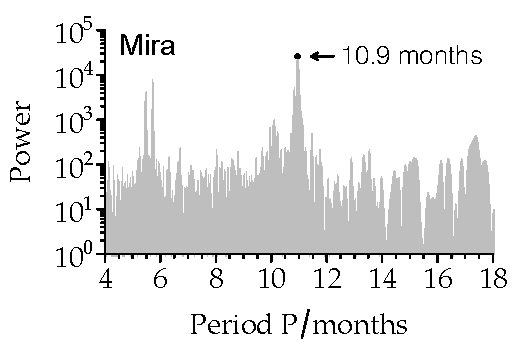
\includegraphics[width=0.5\textwidth]{figs/pgrams/mira_pgram.pdf}%
    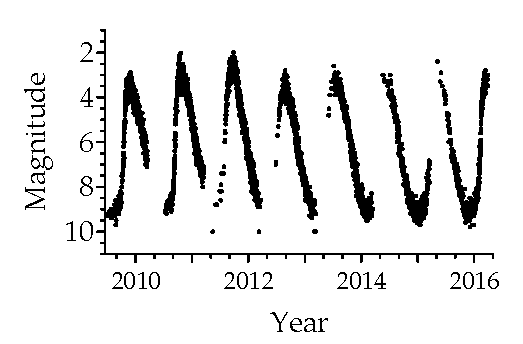
\includegraphics[width=0.5\textwidth]{figs/pgrams/mira_lc.pdf}\\%
    \vspace*{0.4cm}
    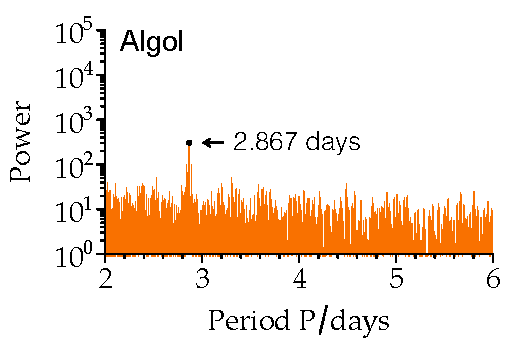
\includegraphics[width=0.5\textwidth]{figs/pgrams/algol_pgram.pdf}%
    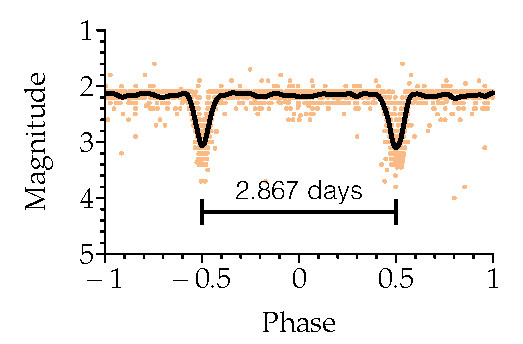
\includegraphics[width=0.5\textwidth]{figs/pgrams/algol_phased.pdf}\\%
    \vspace*{0.4cm}
    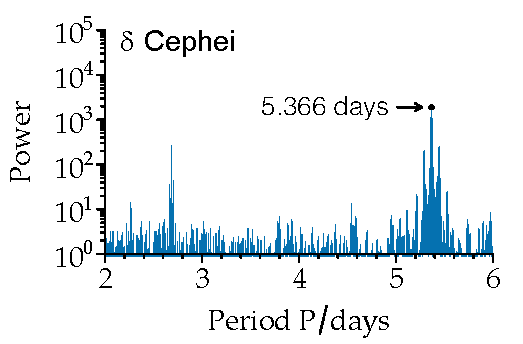
\includegraphics[width=0.5\textwidth]{figs/pgrams/dcep_pgram.pdf}%
    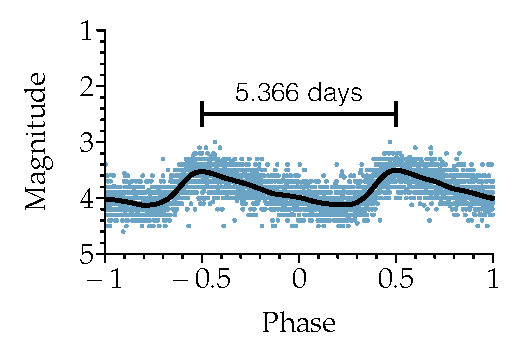
\includegraphics[width=0.5\textwidth]{figs/pgrams/dcep_phased.pdf}\\%
    \vspace*{0.4cm}
    \caption[Light curves of the first-known periodic variable stars]{Modern-day periodograms and light curves for Mira ($o$~Ceti), Algol ($\beta$~Persei), and $\delta$~Cephei---the ``prototypes'' for the first three discovered classes of periodic variable stars. 
    The light curves for Algol and $\delta$~Cephei are phased by their period. 
    Mira has a long and somewhat irregular period. 
    Unlike the other two, which are constantly changing in brightness, the light from Algol is generally stable with occasional quick dips. 
    %Unlike the other two, Mira has a long and somewhat irregular period. 
    %Whereas Mira and $\delta$~Cephei are constantly changing in brightness, the light from Algol is generally stable with occasional quick dips. 
    \emph{Data acquired from the American Association of Variable Star Observers} \citep[\textsc{AAVSO},][]{AAVSO}. 
    \label{fig:lightcurves}}
\end{figure}

For a long time thereafter, the discovery of variable stars slowed. 
Less than ten new variables were discovered in the following $60$ or so years. 
These new variables were published by the German astronomer Friedrich Wilhelm Argelander \citep{1844scja.book..122A}, to whom the variable star naming convention\footnote{ Starting with the letter R and the name of the constellation where it is found (e.g., R~Lyrae), then repeating with double letters when the alphabet is exhausted (e.g., RR~Lyrae).} is owed.
The only other major advance in the first half of the 19th century was the development of the least squares method, which improved period estimates \citep[e.g.,][]{1994JHA....25...92Z}. 

In the second half of the 19th century, the fields of astronomical spectroscopy and dry plate astrophotography were born. 
These technologies proved a great aid for the discovery and analysis of variable stars, and even revealed the existence of several new classes of variable stars. 
By 1865, the number of known variable stars had more than doubled, going up to $123$ \citep{1865AN.....63..117C}. %\citep{1958HDP....51..353L}. 
In the next $30$ years, that number quadrupled with over $300$ new discoveries \citep[e.g.,][]{1997JAVSO..25..115H}. 
Nearly $50$ variable stars were discovered in the year 1896 alone, the majority of which being Mira-type variables, $19$ of which were found by the Harvard ``computer'' Williamina P.~Fleming. 
By the end of the 19th century, the number of known variable stars grew to at least $2000$ \citep[e.g.,][]{Samus2017}. %; and by 1915, nearly 14000 \citep{1958HDP....51..353L}. 

% 1868 helium discovered in the Sun 

%\subsection*{Theoretical Developments}

The latter half of the 19th century also marked the beginning of a change in attitude toward astronomical research. 
In addition to cataloging the sky, researchers began seeking rigorous physical foundations to understand the nature of the Sun and the stars. 
Applying techniques from the recently-born field of thermodynamics, figures such as William Thomson (a.k.a.\ Lord Kelvin), Julius Robert Mayer, Hermann von Helmholtz and others worked to determine the ages of stars and identify the sources of their energy. % such as identifying the sources of their energy and measuring their ages began receiving serious consideration. 
In particular, they offered the explanation that gravitational energy can be converted into heat via either contraction or the infall of meteoric material. 
For example, Helmholtz demonstrated that the Sun could be powered by contracting merely $380$ feet each year \citep[e.g.,][]{ARNY1990211}. 
Now called the Kelvin-Helmholtz mechanism, this was the only known form of stellar heating at the time. 
Applying it to the study of the Earth and Sun, Kelvin found that the solar system must be at most millions of years old \citep[e.g.,][]{1895Natur..51..438K}, much younger than the currently accepted age of about $4.57$ billion years.\footnote{ A devout Christian, Lord Kelvin used these results to doubt Charles Darwin's recently-published theory of biological evolution, which requires an older Earth \citep{darwin}.}
%The Kelvin-Helmholtz mechanism would remain the only accepted form of stellar heating for decades. 

The calculations that Helmholtz and Kelvin made required details of the structure of the Sun, and so to carry them out, they created the first polytropic models of stellar structure \citep[e.g.,][]{ARNY1990211}. 
These models are characterized by the internal pressure depending only on the density of the stellar material. 
Much as is still done today, they considered a sphere where gravity forces are in balance against pressure forces. 
However, they erroneously assumed that all energy in the Sun is transported by convection. 
%They assumed all energy in the Sun is transported by convection, which is difficult to work out. 
%They the first \emph{polytropic} models, which are characterized by the internal pressure depending only on the density of the stellar material. 
%They assumed that all the energy would be transported by convection, which is difficult to work out, so they developed models that did not require such information. 
%The types of models they developed are called polytropes, which are characterized by the internal pressure depending only on the density of the stellar material. 
%characterized by the pressure throughout the interior depends exclusively on the density. 

It was also around this time that the idea stars might pulsate was first given serious attention. %the theory of stellar pulsations began being fleshed out. 
Lord Kelvin was the first to state the equations of non-radial pulsation for chemically homogeneous ``spheroids of incompressible liquid'' \citep{1863RSPT..153..583T}. 
Though this work makes no explicit mention of stars, it was thought at this time that stars might be entirely liquid \citep[e.g.,][]{ARNY1990211}. 
However, it was argued for a long time thereafter that stars could not possibly pulsate non-radially, as these modes of oscillation would be damped out by viscous forces \citep[e.g.,][]{1938ApJ....88..189P}. 
Figure~\ref{fig:sph} shows some of the configurations that a star could take under the pulsation hypothesis. 


\begin{figure}
    \centering
    %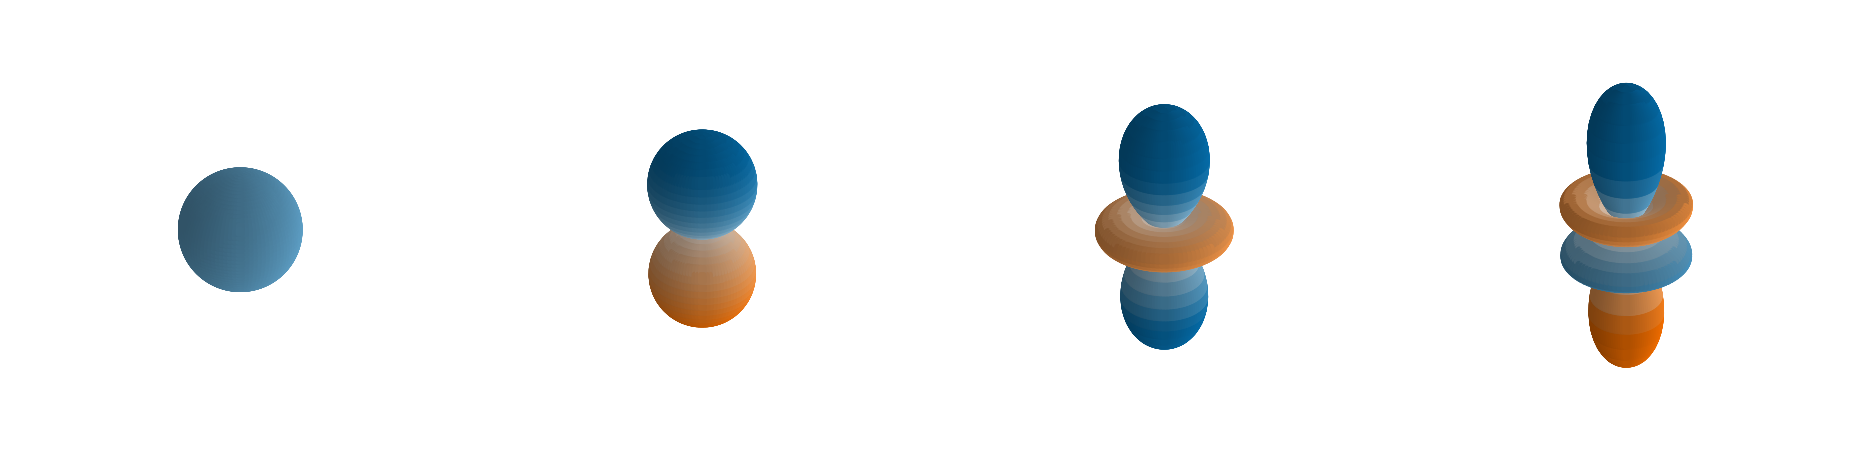
\includegraphics[width=\textwidth]{figs/pulse/sph/sph.png}%SphericalHarmonics.png}
    \begin{overpic}[width=\textwidth,trim={0 0.5cm 0 0}, %0.5cm},%,
                clip%,tics=10,grid
            ]{figs/pulse/sph/sph.png}
        \put (9,19)  {\text{radial}}
        \put (33.8,19) {\text{dipole}}
        \put (55.6,19) {\text{quadrupole}}
        \put (82.1,19) {\text{octupole}}
    \end{overpic}
    \caption[Spherical harmonics]{\lr{Radial and non-radial stellar pulsations for a non-rotating star. 
    Mathematically, these show ${r(\theta, \phi) = \Re |Y_{\ell}(\theta, \phi)|}$ in spherical polar coordinates for ${\ell=0}$, $1$, $2$, $3$, where $Y_{\ell}$ is the solution to Laplace's equation on a sphere---special functions known as \emph{spherical harmonics}. The sign of ${\Re(Y_{\ell})}$ is indicated by color. 
    %Mathematically, these are the real solutions of $|Y_{\ell}|$ for degrees ${\ell=0,1,2,3}$ to Laplace's equation on a sphere---special functions known as \emph{spherical harmonics}. 
    %The sign of the function is indicated by the color. 
    %The figure shows $|\text{Re}\{Y_\ell\}| [x,y,z]$ in spherical coordinates, with the sign of the function indicated with color. %, with the sign of the function indicated by the color. 
    %These are solutions to Laplace's equation, known as \emph{spherical harmonics}, which are the (exaggerated) 
    Pulsations with ${\ell=0}$ correspond to the entire star moving toward or away from the center without horizontal motions, i.e., radial pulsations.}
    %The distance from the center is the value of $Y_{\ell}$. 
    %Pulsations with $\ell>0$ have horizontal and radial motions alike and are called non-radial pulsations. 
    %The modes with $\ell>0$ are non-radial. 
    %radial ($\ell=0$), dipole ($\ell=1$), quadrupole ($\ell=2$) and octupole ($\ell=3$) oscillations, where $\ell$ is the spherical degree of the mode. 
    \label{fig:sph}}
\end{figure} %% TODO: EXPLAIN PLOT 


%, when Ernest Rutherford suggested that the recently-discovered mechanism of radioactive decay could heat the Sun \citep{}. 

After completing his Ph.D.\ at the University of G\"ottingen, the German astrophysicist August Ritter wrote a series of $19$ papers over an $11$-year span laying out theory of stellar structure \citep[1878--1889, e.g.,][]{ritter}. 
%Treating stars as an ideal gas, he worked out a differential equation describing the density of a star as a function of radius (now called the Lane--Emden equation) and derived a relationship between the mass of a star and its luminosity. 
Ritter had the insight to treat stars as an ideal gas, and derived a relationship between the mass of a star and its luminosity. 
Ritter also developed here the radial theory of stellar pulsations, including the important result connecting the period of stellar pulsation to the mean density of the star. 
Since the source of stellar variability was still an open puzzle, Ritter conjectured that stars might be radial pulsators. 
Unfortunately, this work was largely ignored.\footnote{ In his influential textbook \emph{An Introduction to the Study of Stellar Structure}, Nobel laureate \citet{1939isss.book.....C} characterized this body of work as ``a classic, the value of which has never been adequately recognized,'' and noted that in these works Ritter worked out ``almost the entire foundation for the mathematical theory of stellar structure.''} 
%Many of Ritter's ideas were reviewed in Robert Emden's influential monograph on polytropes ``Gaskugeln'' \citep[literally ``gas balls,''][]{emden1907gaskugeln}. 

In an attempt to understand the temperature of the Sun, the American theoretical astrophysicist and Yale alumnus J.\ Homer Lane continued work on polytropes \citep[e.g.,][]{1870AmJS...50...57L}. 
Lane discovered the curious fact that stars have a negative heat capacity: i.e., when they lose energy, they contract and heat up. 
%This came to be known as \emph{Lane's Law}, and would soon inspire the first physical theory of stellar evolution. 
Ritter rederived Lane's Law and used it to develop the first physically-motivated (albeit incorrect) theory of stellar evolution: that a star begins its life as a diffuse gaseous mass, which at first contracts and heats; eventually, the star transforms into a liquid, and then undergoes a long period of cooling. 
%This theory, now regarded as essentially incorrect---or, at a bare minimum, missing many details in between---was enthusiastically championed by the influential English scientist Norman Lockyer \citep[e.g.,][]{ARNY1990211}, famous for discovering helium in the Sun \citep[e.g.,][]{10.2307/109002} and for founding the journal \emph{Nature}. 
%It thus held prominence for decades to come. 

%\subsection*{}

At the end of that century, the German astronomer Hermann Carl Vogel used spectroscopic measurements to firmly establish that Algol is an eclipsing binary, thereby confirming Goodricke's initial speculation \citep{1889AN....121..241V, 1908ApJ....27....1F}. 
%Not long thereafter, Mira too was found to be a double star \citep{1923PASP...35..323A}.
%However, being that its companion has an orbital period of nearly 500 years, that did not explain its 11-month variations. though the dynamics and configuration of such a system were difficult to explain. 
Vogel taught his methods to the Russian astronomer Aristarkh B{\'e}lopolsky, who then took spectra of the Cepheid stars $\delta$~Cephei and $\eta$~Aquilae. 
Though at this time eclipses were widely thought to be the most likely the source of Cepheid variability, B{\'e}lopolsky argued that the radial velocity variations of these stars were inconsistent with the eclipse hypothesis \citep{1897ApJ.....6..393B, 1895ApJ.....1..160B}. 
\epigraph{``\emph{The times of minimum brightness and the times for which the velocity in the line \hphantom{``}of sight is zero do not coincide. For this reason the changes in the brightness of \hphantom{``}the star cannot be explained as the result of eclipses, and some other explanation \hphantom{``}must be sought.}''}{--- Aristarkh Apollonovich B{\'e}lopolsky \\\textit{Researches on the spectrum of the variable star $\eta$~Aquilae} (\citeyear{1897ApJ.....6..393B})}

Several alternative theories for Cepheid variability arose over the years. 
So-called ``veil theories'' suggested that clouds could rapidly form and evaporate, serving to block the source of the light for a short time \citep[e.g.,][]{1889Natur..39..606B}. 
%However, it was difficult to formulate a physically-motivated model to justify the periodic formation and dissipation of clouds around a star \citep[e.g.,][]{1958HDP....51..353L}. 
English astronomer Henry Plummer, later President of the Royal Astronomical Society, suggested that Cepheids are radial pulsators \citep{1914MNRAS..74..660P}. 
%Many, including the eminent star formation theorist James Jeans, rejected the pulsation hypothesis, Jeans himself arguing that Cepheid variation is rather caused by repeating explosions \citep[e.g.,][]{1919Obs....42...88J}. 
Others maintained the eclipsing binary hypothesis \citep[e.g.,][]{1909LicOB...5...82D} with some even claiming that B{\'e}lopolsky's measurements had in fact proven it \citep[e.g.,][]{1913Obs....36...59B}. 

Regardless of the cause of their blinking, Cepheid stars gained near-immediate fame throughout astronomical circles and beyond following the discovery by American astronomer Henrietta Swan Leavitt (another Harvard `computer') that ``the brighter variables have the longer periods'' \citep{1908AnHar..60...87L, 1912HarCi.173....1L}. 
Now known as the Cepheid Period-Luminosity Relation or the \emph{Leavitt Law}, this enabled measurement of vast cosmic distances via comparison of observed brightnesses with those expected from Cepheid periods. 
This discovery thus established Cepheids as standard candles---the first to be discovered---and was quickly put to use in mapping the structure of the Universe (see Figure~\ref{fig:var-day}). 

%longer-period Cepheids are more luminous than the shorter-period ones, 
%Now known as the Cepheid Period-Luminosity Relation or the \emph{Leavitt Law}, comparison of the observed brightness with that expected from the period. 
%This discovery established Cepheids as standard candles---the first to be discovered---and thus enabled measurements of vast cosmic distances (see Figure~\ref{fig:var-day}). 


%\iffalse
%\epigraph{\emph{``It is worthy of notice that the brighter variables have the longer periods.''}}{Henrietta Swan Leavitt \\\textit{1777 Variables in the Magellanic Clouds} (\citeyear{1908AnHar..60...87L})}
%\fi
%\noindent 

%\iffalse
\begin{figure}
    \centering
    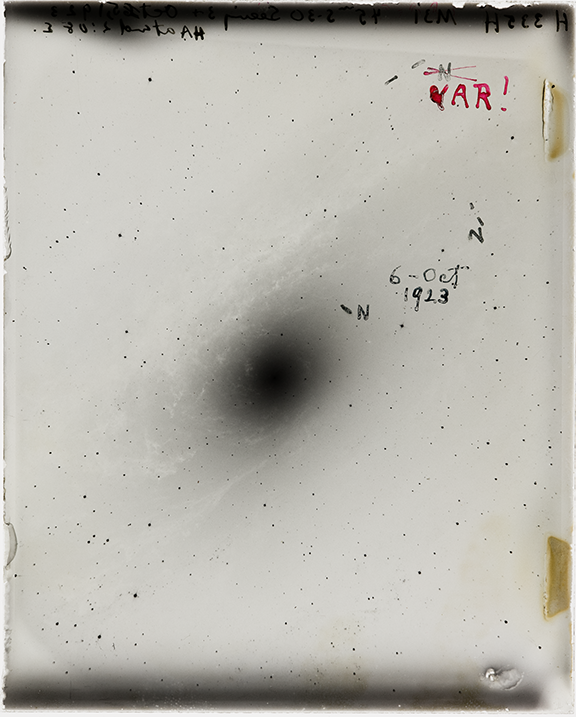
\includegraphics[width=\textwidth,trim={0 5cm 0 2cm},clip]{pics/var3.png}
    \caption[VAR! Day]{Edwin Hubble's photographic plate showing the discovery of a Cepheid variable star in the Andromeda Galaxy (M31). 
    In a series of $17$ papers, Harlow Shapley used the Leavitt Law to estimate the distance to globular clusters and map out the size of the Galaxy, finding that it was substantially larger than previously estimated \citep{1918ApJ....48...89S}. 
    In 1920, Shapley engaged in the ``Great Debate'' of astronomy, in which he argued that the Milky Way comprised the entirety of the Universe \citep{1921BuNRC...2..171S}. 
    Soon thereafter, Edwin Hubble used this same technique to measure the distance to the spiral nebulae M31 and M33 \citep[][see image]{1925Obs....48..139H}. 
    Finding that they were extremely distant, Hubble proved that these nebulae were in fact galaxies external to our Milky Way---instantly expanding the calculated size of the Universe by a factor of $100,000$. 
    Hubble sent these results to Shapley, who, upon viewing them, is said to have remarked: \emph{``Here is the letter that has destroyed my Universe.''} 
    Edwin Hubble subsequently used the Leavitt Law to estimate the distances to several more Cepheid-host galaxies \citep{1929PNAS...15..168H}. 
    Combining these distances with measurements of the speeds at which those galaxies are receding from us, Hubble measured the rate of cosmic expansion, and thus the age of the Universe. 
    Variable star enthusiasts can celebrate October 6 as ``VAR! Day'' (see image). 
    \emph{(Image reprinted with permission from Carnegie Observatories.)}
    \label{fig:var-day}}
\end{figure}
%\fi
%\subsubsection*{Dwarfs and Giants}

Around this time, the then-unknown Danish astronomer Ejnar Hertzsprung was working to combine spectroscopy of stars with parallax distance measurements. 
He found that stars form two distinct groups: ``Riesen'' (giants) and ``Zwerge'' (dwarfs). 
Hertzsprung published this work in a photographic journal with little impact \citep{1905WisZP...3..442H, 1907WisZP...5...86H}. 
It did however get the attention of Karl Schwarzschild, director of the G\"ottingen Observatory, who then appointed him to a position there \citep[e.g.,][]{bolt2007biographical}. 
Hertzsprung went on to discover that the pole star Polaris is also a Cepheid-type variable\footnote{ Hence, Caesar is as constant as a variable star \citep{shakespeare}.} \citep{1911AN....189...89H} and furthermore concluded that Cepheids are giant stars \citep{1913AN....196..201H}. 

The director of the Princeton Observatory, Henry Norris Russell, a much more influential astronomer at the time, also came to the same conclusions as Hertzsprung \citep[e.g.,][]{1913Obs....36..324R, 1913Sci....37..651R}. 
Plotting the absolute magnitudes of more stars against their spectral type (see Figure~\ref{fig:HRD}), Russell showed that there was a main diagonal where dwarfs lived, an upper corner where red giants lived, and a lower corner lacking any stars ``except for one star\footnote{ This would later be recognized the first-discovered white dwarf \citep[e.g.,][]{1958whdw.book.....S}.} whose spectrum is very doubtful.'' 
Russell argued that this confirmed Ritter's theory of evolution. 
%Russell furthermore argued that this had observationally confirmed the then-prevailing theory of stellar evolution: that stars begin their lives as gaseous red giants, and then compress and heat until they become liquid dwarfs, at which point they cannot compress anymore, so they cool. 

\begin{figure}
    \centering
    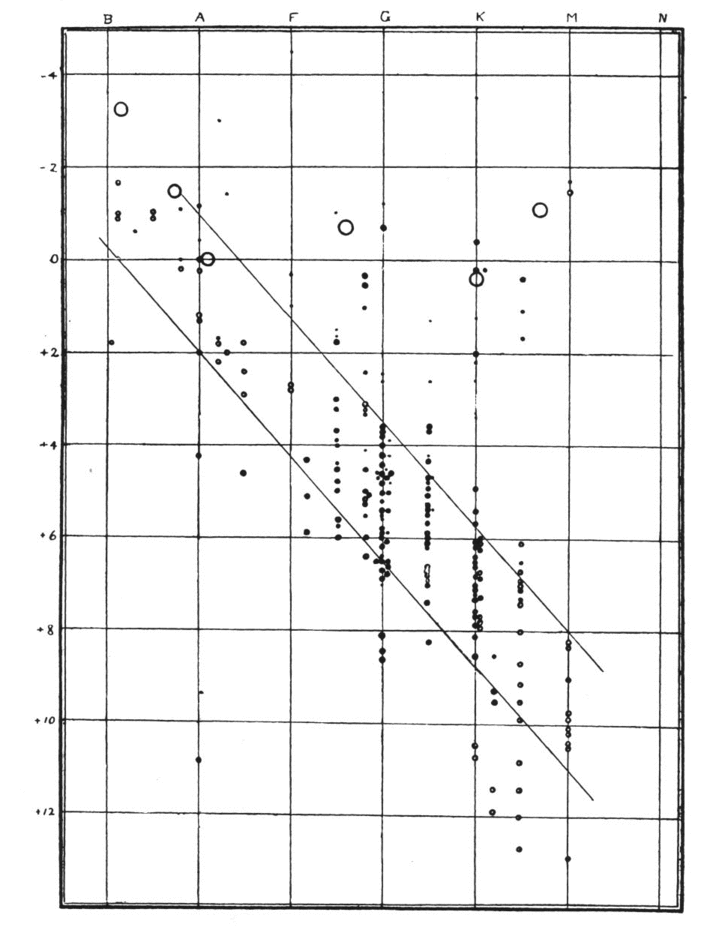
\includegraphics[width=\textwidth]{pics/old_hr.png}
    \caption[Historical Hertzsprung-Russell Diagram]{One of the first Hertzsprung-Russell diagrams, showing the absolute magnitude of stars against their spectral type. 
        Luminosity increases upward; temperature increases leftward. 
        Dwarf stars reside on the diagonal---the \emph{main sequence}---and giant stars occupy the upper right corner. 
        \emph{(Figure reprinted with permission from \citealt{1914Natur..93..252R}.)} 
        \label{fig:HRD}}
\end{figure}


%\subsubsection*{Stellar Pulsations}

The following year, Harlow Shapley wrote a seminal paper laying out the collective arguments against the eclipsing binary hypothesis of Cepheid variable stars \citep{1914ApJ....40..448S}. 
First, B{\'e}lopolsky had already shown that the brightness and radial velocity variations did not coincide. 
Second, the periods of some Cepheids are themselves variable. %\citep[e.g.,][]{1916ApJ....43..217S},
Third, the shapes of the light curves for some Cepheids change from cycle to cycle \citep[e.g.,][]{1905ApJ....22..274C}. 
And lastly, ``the best argument,'' since Hertzsprung and Russell had just shown that Cepheids are giant stars, the companion star would need to be inside of the Cepheid in order for eclipses to explain the observed behavior---a ridiculous hypothesis. 
%Shapley concurred with Plummer that the variability of Cepheid stars is most likely due to pulsation.
Shapley concluded that Cepheid variability is most likely due to pulsation.\footnote{ It is interesting to note here that John Michell had posed both the theory of earthquakes \citep{Michell01011759} and the explanation of stellar variability in terms of eclipsing stars \citep{michell1767inquiry}, but probably never imagined that stars quake, too.}  

%Shapley concluded that Cepheid variability is most likely due to pulsation.
\epigraph{``\emph{Cepheid variables are not binary systems... the explanation of their light-changes \hphantom{``}can much more likely be found in a consideration of internal or surface pulsations \hphantom{``}of isolated stellar bodies.}''}{--- Harlow Shapley\\\textit{On the Nature and Cause of Cepheid Variation} (\citeyear{1914ApJ....40..448S})}
%\noindent Thus the pulsation hypothesis was born. 
%Shapley further reminded readers that if a star is indeed pulsating, then timing its pulsations then gives a proxy for the stellar mean density. 

Thus the pulsation hypothesis was born. 
But the theory had its doubters. 
There was no real proof yet---only very strong evidence that the eclipsing binary hypothesis was wrong---and no known mechanism for the pulsation. 
Many, including the eminent star formation theorist James Jeans, rejected the idea of stellar pulsations, Jeans himself arguing that Cepheid variation is rather caused by repeating explosions \citep[e.g.,][]{1919Obs....42...88J}. 
Moreover, many aspects of stellar theory still had major flaws. 
It was still not yet discovered how stars really get their energy, nor how they transport it throughout the interior, nor what they are made of, nor what state of matter they are in, nor how they evolve. 
Jeans himself in fact still held the view that stars are liquid \citep[e.g.,][]{1928Natur.121..173J}. 
%, and with it came great new insights into the nature of the stars. 
%The theory did have its doubters, but observational confirmations would continue to come over the years. 
%\footnote{ Though in this paper Shapley quotes at length works written in German, he makes no indication that he was aware of Ritter's earlier work on stellar pulsations.} 

The modern view of the stars really began to take hold in the early 20th century with the work of Arthur Eddington. 
Building upon earlier works by \citet{Schwarzschild1906} and \citet{1895MmRAS..51..123S}, Eddington developed the first models of radiative transport in stellar interiors \citep[e.g.,][]{1916MNRAS..77...16E}. 
Combating the view that stellar energy is transported entirely by convection, Eddington worked out the balance between radiative pressure---the outward pressure exerted by the enormous numbers of photons streaming through the star---with the inward pressure exerted by the gaseous stellar material. 
This led to the creation of his ``standard model''---a purely radiative star. 
%Eddington worked out the balance between gas pressure and radiative pressure, and provided an approximate description of stellar atmospheres. %that is still in use today. 
This treatment complicated stellar models greatly, as the internal structure then depended on the opacity and mean molecular weight of the stellar matter, which were unknown \citep[e.g.,][]{ARNY1990211}. 

%eddington mechanism. baade-wesselink proof. Interestingly, John Michell had posed both the theory of earthquakes (\citeyear{Michell01011759}) and the theory of eclipsing stars (\citeyear{michell1767inquiry}), but did not live long enough to find out that stars quake, too. 

The following year, Eddington provided the mechanism for Cepheid variability \citep{1917Obs....40..290E}. 
Applying thermodynamics to the study of the interior, Eddington argued qualitatively that Cepheids pulsate due to an internal heat engine: repeated expansion and collapse due to cyclical ionization and recombination of atoms. 
The following year, he numerically calculated the periods of his stellar models using a linear adiabatic treatment of stellar pulsation, and found good agreement with observations \citep{1918MNRAS..79R...2E}. 
Though further confirmations would come later, this was already strong evidence for the pulsation hypothesis.%did not live long enough to find out that stars quake, too. 

Eddington then went on to use observations of Cepheids to dispute the Kelvin-Helmholtz mechanism as being the sole source of stellar longevity \citep{1920SciMo..11..297E}. 
If stars survive on contraction alone, he argued, then their rate of rotation should speed up relatively rapidly due to the conservation of angular momentum. 
This was not what had been observed. 
Similarly, if the pulsation hypothesis is true, then their period of pulsation should change in accordance with changes to their mean density. 
\epigraph{``\emph{Now, on the contraction hypothesis the change of density must amount to at least \hphantom{``}1 per cent.\ in 40 years. The corresponding change of period should be very easily \hphantom{``}detectable. For $\delta$~Cephei the period ought to decrease 40 seconds annually. Now \hphantom{``}$\delta$~Cephei has been under careful observation since 1785, and it is known that \hphantom{``}the change of period, if any, must be very small. S.~Chandler found a decrease of \hphantom{``}period of 1/20 second per annum... I hope the dilemma is plain... Only the inertia \hphantom{``}of tradition keeps the contraction hypothesis alive---or rather, not alive, but an \hphantom{``}unburied corpse.}''}{--- Sir Arthur Stanley Eddington \\\emph{The Internal Constitution of the Stars} (\citeyear{1920SciMo..11..297E})} 

%Thus the Kelvin-Helmholtz mechanism was out. 
Eddington furthermore rederived Ritter's mass-luminosity relation, and upon applying the relation to stars of spectral types B and A, found that these ``dwarf'' stars are even more massive than the giant stars \citep[e.g.,][]{1924MNRAS..84..308E}. 
This too was difficult to reconcile with the prevailing theory of stellar evolution. 
%Thus, both the Kelvin-Helmholtz mechanism and Lane's Law were out. 

Eddington therefore sought another explanation. 
During Albert Einstein's ``miracle year,'' Einstein had given his famous equivalence of mass and energy, ${E=mc^2}$ \citep{1905AnP...323..639E}. 
%Eddington served as Secretary of the Royal Astronomical Society during the first world war, and was thus among the first to receive notice of Einstein's developments \citep[e.g.,][]{bolt2007biographical}. %was one of few astronomers who closely followed the highly mathematical developments in theoretical physics, Eddington worked to apply these to the theory of stellar interiors. 
%Eddington became a champion of Einstein's work, writing several articles and books on relativity theory \citep[e.g.,][]{1920stga.book.....E}, and providing convincing evidence for the theory by observing the deflection of light in the solar eclipse of 1919 \citep{1920SciMo..10...79T}. 
%
%
%Eddington sought to apply Einstein's work to the study of the stellar interior, and in 1920, the English chemist and Nobel laureate Francis Aston supplied an essential ingredient. 
In 1920, the English chemist and Nobel laureate Francis Aston showed that the mass of one helium atom was approximately $1\%$ less than the sum of four hydrogen atoms \citep{aston1920lix}. 
At this time, it was still assumed that the solar composition was similar to that of the Earth; the amount of hydrogen in the Sun was therefore thought to be relatively small. 
Nevertheless, and despite lacking an exact mechanism, Eddington used these two developments to speculate that the Sun and stars survive via hydrogen fusion \citep{1920SciMo..11..297E}. 
\epigraph{``\emph{A star is drawing on some vast reservoir of energy by means unknown to us. \hphantom{``}This reservoir can scarcely be other than the sub-atomic energy which, it is \hphantom{``}known, exists abundantly in all matter; we sometimes dream that man will one \hphantom{``}day learn how to release it and use it for his service... The atoms of all elements \hphantom{``}are built of hydrogen atoms bound together, and presumably have at one time \hphantom{``}been formed from hydrogen; the interior of a star seems as likely a place as any for \hphantom{``}the evolution to have occurred; whenever it did occur a great amount of energy \hphantom{``}must have been set free; in a star a vast quantity of energy is being set free which \hphantom{``}is hitherto unaccounted for.}''}{--- Sir Arthur Stanley Eddington \\\emph{The Internal Constitution of the Stars} (\citeyear{1920SciMo..11..297E})} 

Within five years, Harlow Shapley's Ph.D.\ student Cecilia Payne showed that hydrogen is about a million times more prevalent in the Sun and stars than on the Earth \citep{1925PhDT.........1P}.
Within two years, the G\"ottinger physicist Friedrich Hund discovered quantum tunnelling, which gives atomic nuclei a probability of penetrating the Coulomb barrier and achieving thermonuclear fusion \citep{hund1927deutung,Nimtz2009}. 
The following year, George Gamow brought this concept to the astrophysical community \citep{1928Natur.122..805G}, and Eddington's speculation was proved. 
Eddington calculated new stellar models that included hydrogen burning, and found that this mechanism could power the Sun for billions of years \citep{1926ics..book.....E}. 

This was not the end of the story, however. 
Though hydrogen fusion was now known to fuel the stars, there were still major discrepancies between theory and observation. 
Using the assumption that the stellar interior is chemically homogeneous, George Gamow calculated evolutionary tracks and found that his models failed to become giant stars \citep[][see also Figure~\ref{fig:gamow-tracks}]{1938PhRv...53..907G}.
He furthermore found that he could not reproduce the mass-luminosity relation. 
%Figure~\ref{fig:gamow-tracks} shows George Gamow's evolutionary tracks from the late 1930s, where Gamow has incorrectly assumed that the stellar interior is chemically homogeneous \citep{1938PhRv...53..907G}. 
%All of the tracks failed to evolve into giant stars, leaving the origin of the giants a mystery. 
%Furthermore, there are substantial disagreements with the mass-luminosity relation. 

\begin{figure}
    \centering
    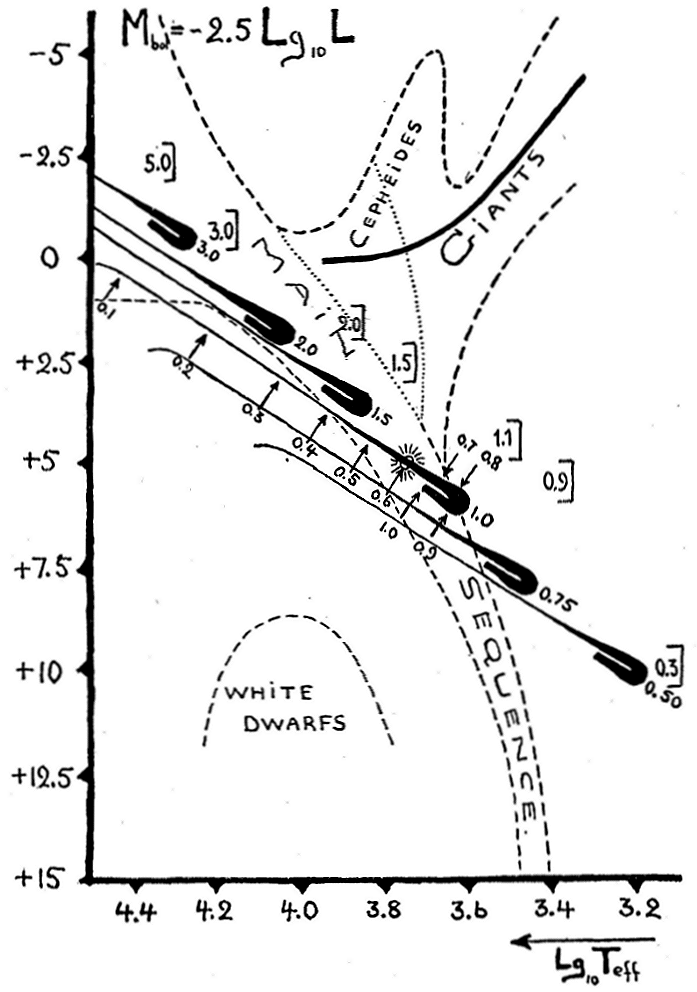
\includegraphics[width=0.75\textwidth]{ch1_introduction/pics/gamow-tracks.png}
    \caption[Historical theoretical H-R diagram]{
        Historical theoretical Hertzsprung-Russell diagram showing the evolution of stars with initial masses spanning from $0.5$ to $3$ solar masses. 
        The thickness of each track indicates the time spent at that stage of evolution. 
        The arrowed numbers indicate the amount of hydrogen. 
        The numbers in brackets indicate masses obtained via the mass-luminosity relation. 
        Unlike modern evolutionary tracks, the stars simulated here fail to evolve from dwarfs into giant stars. 
        \emph{(Figure reprinted with permission from \citealt{1938PhRv...53..907G}.)}
    \label{fig:gamow-tracks}}
\end{figure}

The solution came that same year, though it would not be widely recognized until long after. 
Discarding Gamow's mixing hypothesis, the Estonian astrophysicist Ernst \"Opik realized that hydrogen fusion could continue burning in a shell after it had been exhausted in the core. 
Applying this insight, \"Opik succeeded in hand-calculating stellar models that evolve from the main sequence up the red giant branch \citep{1938PTarO..30C...1O}. 
Thus, the major features of the H-R diagram were explained. 
Unfortunately, it would be decades before this solution was rediscovered using digital computers \citep[e.g.,][]{ARNY1990211}. 
Although there was still much to do about the evolution beyond the red giant branch---and although debates continue to this day over why stars actually become giants \citep[e.g.,][etc.]{10.1007/978-94-009-8492-9_18,1992ApJ...400..280R,1983A&A...127..411W,1985ApJ...296..554Y,1988ApJ...329..803A,1989MNRAS.236..505W,1991AnPh...16..515W,2000ApJ...538..837S}---this essentially captured the first phases in the modern picture of stellar evolution. 


%Eddington also gave a mechanism for Cepheid pulsations in terms of a `heat engine' wherein stars expand and collapse due to cyclical ionization and recombination of atoms, which remains the accepted explanation. 
%In this book, Eddington repeated the then-prevailing theory of stellar evolution: that stars begin as giants and end their lives at dwarfs, only now (correctly) adding that they eventually become white dwarfs. 
%stated the prevailing theory of stellar evolution of the time: stars begin their lives on the giant branch, and lose mass or otherwise collapse onto the main sequence as dwarf stars, and eventually end their lives as white dwarfs. 
%In the year of the book's release, Heinrich Vogt stated his \emph{Eindeutigkeitssatz} (uniqueness theorem), also known as the \emph{Vogt-Russell theorem}: that the structure of a star is uniquely determined by its mass and chemical composition \citep{1926AN....226..301V}. 
%Though widely believed for a long time, we now know both to be incorrect. 

%Vogt-Russell theorem \citep{1926AN....226..301V} 

%Eddington developed the ``standard model'' to account for the pulsations of Cepheid variable stars. 
%1926 The Internal Constitution of the Stars 
%1913 HR diagram Giant and Dwarf theory 

%Eddington recognized the importance of radiative equilibrium %balancing %radiation pressure---the pressure exerted by the enormous numbers of photons streaming through the star---with the pressure of th. 

There was still one more major hitch that needed to be reconciled. 
Around the same time that these issues were being resolved, the German-born American astronomer Edward Arthur Fath discovered that $\delta$~Scuti---a star with much resemblance to the Cepheids---has more than one period of pulsation \citep{fath1935photometric}. 
This brought serious challenges to the theory of stellar pulsation, as the second period measured was inconsistent with the mean density of the star \citep{1938ApJ....87..133S,1940PNAS...26..537S}. 
\epigraph{``\emph{One is practically forced to the conclusion that the existence of the pair of periods \hphantom{``}would be inconsistent with the pulsation theory... If the [second period] is correct, \hphantom{``}the pulsation theory is seriously jeopardized.}''}{--- Theodore Eugene Sterne\\\textit{The Secondary Variation of $\delta$~Scuti} (\citeyear{1938ApJ....87..133S})}

Sterne's argument rested on the longstanding assumption that these modes of pulsation needed to be purely radial in nature. 
%Rather than motions driving purely toward or away from the core of the star, one can also consider non-radial pulsations, i.e., waves that additionally have a horizontal component to their motion (see Figure~\ref{fig:sph}). 
%It had so far been assumed that non-radial oscillations would be so viscously damped as to not vibrate at all. 
Challenging this view, \citet{1938ApJ....88..189P} continued Lord Kelvin's work from $75$ years prior to further flesh out the mathematics of non-radial stellar pulsations, only now dealing with heterogeneous chemical compositions---a much more difficult problem. 
\citet{1941MNRAS.101..367C} used this description to calculate the non-radial pulsation frequencies of a stellar model (though his attention was toward binary interactions). %under the now-dubbed ``Cowling Approximation'' 
Such calculations would prove invaluable in the decades to come, as it would be applied to a much more familiar star: the Sun. %with helioseismology and, now, asteroseismology. 
%These calculations would then be applied to 
%Such calculations would later be applied, perhaps surprisingly, to a much more familiar star. 

%something about convection, something about theory of evolution
%\citep{1949ptvs.book.....R} textbook ``The Pulsation Theory of Variable Stars.''
%\the\textwidth

%\citep{1938ApJ....88..189P} nonradial oscillations of stars % linearized equations governing the nonradial adiabatic pulsations of a spherical star in hydrostatic equilibrium 
%\citep{1941MNRAS.101..367C} cowling approximation, nonradial oscillations of polytropes 
%\citep{1968SvA....11..630V} asymptotic descrption of nonradial oscillations in polytropes 

%Martin Schwarzschild 1961 ``Convection in Stars''
%Martin Schwarzschild 1938 ``On the Light Curves of Cepheids''
%Martin Schwarzschild 1941 ``Overtone Pulsations for the Standard Model''
%Martin Schwarzschild 1948 ``On the Pulsation in the Atmosphere of η Aquilae''
%Martin Schwarzschild 1948 ``On the radial velocity of 63 Tauri''

%Chandrasekhar 1964 variational principle 
%Lynden-Bell \& Ostriker 1967 MNRAS variational principle 
%Clement 1964 non-radial oscillations 
%Petersen 1973 mass and radius from double mode pulsators 
%\citep{1965ApJ...142..229L} variational principle + schwarzschild -> frequencies are stable in convection zones \citep{1958ZA.....46..108B} mixing length theory 


%\citep{1938ApJ....87..133S,1940PNAS...26..537S} 
%\citep{1941ApJ....94..245S} theoretical calculations of overtone pulsations 



\subsection{Helioseismology} 
The theory that stars pulsate---and that they can pulsate non-radially---was most definitively confirmed with the discovery in the 1960s and 1970s that our own Sun is in fact such a pulsator. 
Obviously, the nature of solar pulsations are of a different character than the ones discovered in other stars to have gone unnoticed for so long. 
%The amplitudes of solar pulsations are very small
%Rather than at most three simultaneous large-amplitude modes of pulsation, the Sun oscillates in a superposition of a great number of small-amplitude modes, each excited at random by turbulence in its outer envelope. 
%The subtlety of the solar pulsations can be appreciated by how long it took them to be discovered relative to those in other stars. 

Already in 1916, the $23$-year old Canadian solar astronomer Harry Plaskett had found variations in Doppler velocity measurements of the solar surface from a spectroscopic investigation into the solar rotation rate \citep{1916ApJ....43..145P}. 
Whether these variations were intrinsic to the Sun, or, for example, effects from the Earth's atmosphere were unknown until the work by \citet{1954MNRAS.114...17H, 1956MNRAS.116...38H}. 
Many regard the publication of a ``preliminary report'' by Caltech researchers Robert Leighton, Robert Noyes and George Simon as the birth of helioseismology \citep{1962ApJ...135..474L}. 
In this paper, Leighton and colleagues demonstrated that the Sun has multi-periodic variations on the order of about $5$ minutes (see also Figure~\ref{fig:solar-velocity-fields}). 
They were prescient in their speculation that these variations could be used to determine detailed properties of the Sun, or at least its atmosphere. 
\citet{1968ApJ...152..557F} and others furthermore gave evidence that solar oscillations may not merely be confined to the solar atmosphere, but may instead probe deep into the star. 


\begin{figure}[t!]%[p] 
    \centering
    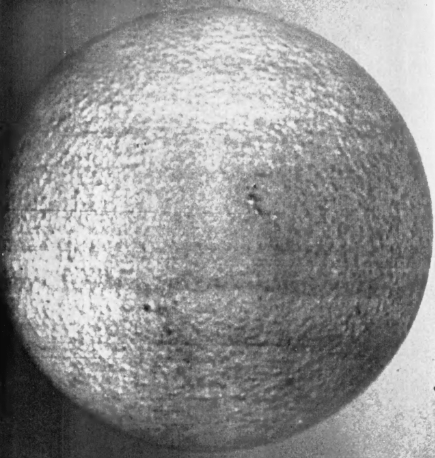
\includegraphics[width=0.66\textwidth,%0.5\textwidth%
        trim={0 1.5mm 0 1.5mm}, clip]{pics/solar-velocity-fields2.png}
    \caption[Velocity fields in the solar atmosphere]{Velocity fields in the solar atmosphere revealed by Doppler imaging. %(June 15, 1960). 
    \emph{(Figure reprinted with permission from \citealt{1962ApJ...135..474L}.)}
    \label{fig:solar-velocity-fields}}
\end{figure}


%Theories to explain the observed solar velocity field soon began to emerge. 
%\citet{1968ApJ...154..297S} derived a theoretical pulsation spectrum by considering wave production by fluid motions. 
%However, the periods of oscillations were off by a factor of five. 
In the early 70s, \citet{1970ApJ...162..993U} and \citet{1971ApL.....7..191L} argued that the oscillations are standing acoustic waves trapped below the solar photosphere, and showed that theoretical periods of this description match the observations. 
\citet{1975A&A....44..371D} and \citet{1977ApJ...218..901R} found that the relationship between the spatial and temporal frequencies of the oscillations are in similar agreement with expectations, giving further credence to the theory. 
\citet{1977ApJ...212..243G} provided a mechanism for the origination of solar oscillations by showing that acoustic waves can be stochastically excited by turbulent convection, which is the dominant source of energy transport in the solar envelope. 
%\citet[e.g.,][]{1975BAAS....7R.478H} gave evidence that the solar diameter is variable, suggesting that the modes are `global' oscillations. 
\lr{\citet{1979Natur.282..591C} and \citet{1980Natur.288..541G} made the first identifications of low-degree modes in the Sun, which pass through the entire star, thereby confirming the global nature of the oscillations (see Figures~\ref{fig:rays} and \ref{fig:solar-power-spectrum}).} 



\begin{figure}[t!]%[p] 
    \centering
    \vspace*{-0.35cm}
    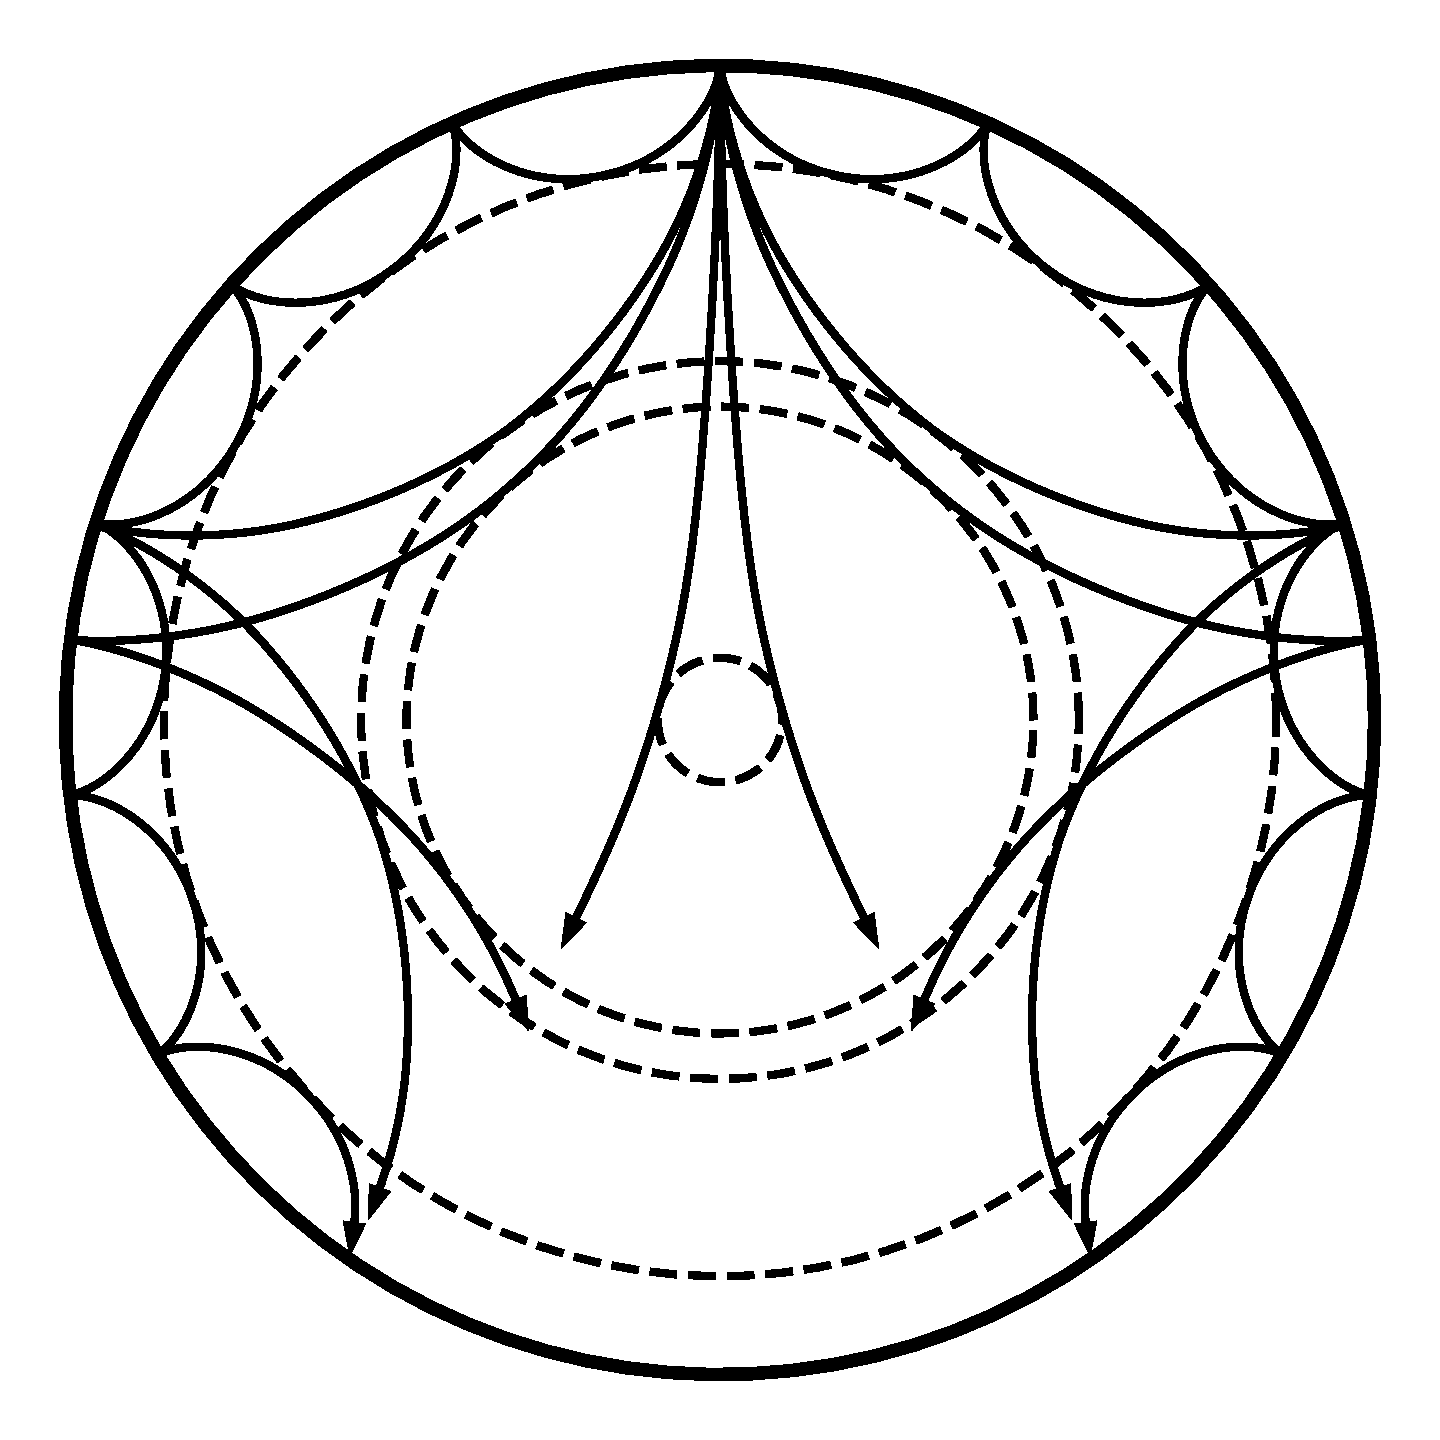
\includegraphics[width=0.73\textwidth%0.48\textwidth%
        ]{figs/pulse/modelS_rays.pdf}
    \caption[Ray path diagram for solar oscillation modes]{Ray diagram showing the paths of oscillation modes as they propagate through the interior of a solar model. 
    The innermost circle shows the lower turning point of a quadrupole (${\ell=2}$) oscillation mode. 
    Such kinds of modes are observable in the Sun and other stars exhibiting solar-like oscillations. 
    The other modes are ${\ell=20}$, $25$, and $75$, which have so far only ever been observed in the Sun. 
    \emph{(Figure adapted with permission from Warrick Ball [private communication] using the procedure given by \citealt{2000PhDT.........9G}.)}
    \label{fig:rays}}
\end{figure}


\begin{figure}
    \centering
    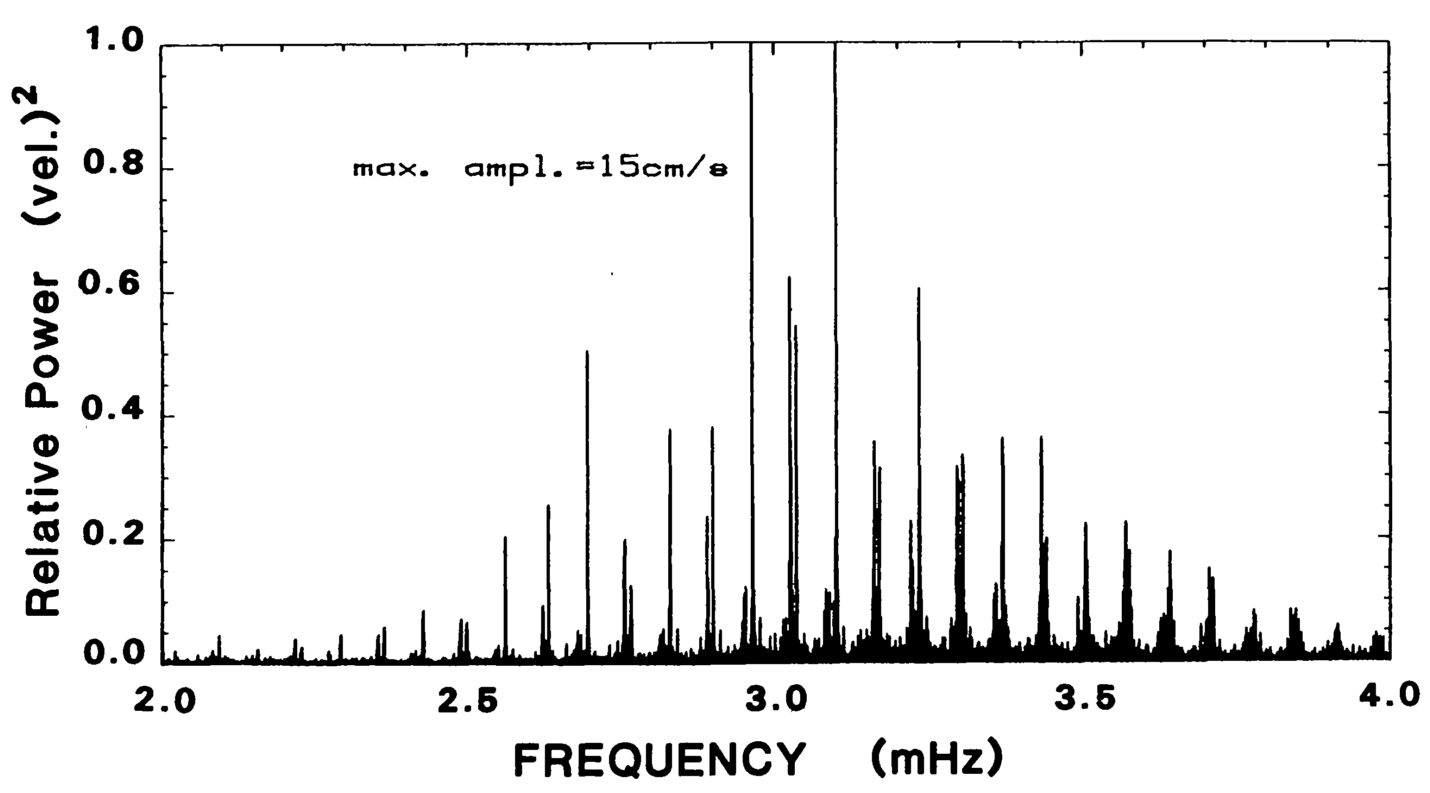
\includegraphics[width=\textwidth]{pics/solar-power-spectrum.png}
    \caption[Historical solar power spectrum]{Power spectrum of the Sun from $3$ months of observations showing its $5$-minute ($3$~mHz) oscillations \citep{1981SoPh...74...51C}. 
    Each peak corresponds to an individual mode of oscillation. 
    \emph{(Figure reprinted with permission from the review article of \citealt{1984ARA&A..22..593D}.)}
    \label{fig:solar-power-spectrum}}
\end{figure}


The Sun vibrates in a superposition of a great number of low-amplitude modes simultaneously. 
Multiple modes of the same spherical degree $\ell$ (recall Figure~\ref{fig:sph}) can be excited simultaneously. 
These modes are distinguished by their radial order $n$, i.e., the number of nodes (zero crossings) between the center and the surface. 
%In the presence of rotation, the modes are split into multiplets distinguished by their 
Additionally, the rotation of the Sun splits each non-radial mode of oscillation into a multiplet of ${2\ell+1}$ modes, which can be distinguished by their azimuthal order $m$, i.e., the number of nodes along the equator. 
%They are further distinguished by the azimuthal order $m$, where $|m|\leq\ell$, which is the number of nodes along the stellar equator. 
%In the absence of rotation, all modes of the same $m$ would have the same frequency. 

Whereas Cepheid and RR~Lyrae stars oscillate in low-order (${n\leq 3}$) radial (${\ell = 0}$) modes, the Sun and other solar-type stars oscillate in high-order (${n\lessapprox 40}$) modes of both radial and non-radial (${\ell\geq 0}$) character, though so far observations of modes with $\ell \geq 4$ have only been confirmed in the Sun, which is made possible by resolving the solar disk. 
Classical pulsators like Mira, Cepheid, RR~Lyrae, and $\delta$~Scuti stars are intrinsically unstable to their oscillations: they are self-excited by their configuration \citep[e.g.,][]{2015EAS....73..111S}. 
Solar-like oscillators, on the other hand, pulsate in stable modes which are both driven and damped by turbulent convection in their outer envelopes. 
Detailed reviews and overviews of global helioseismology have been given by, e.g., \citet{2002RvMP...74.1073C}, \citet{Kosovichev1999,2011lnp...832....3k}, and \citet{2016lrsp...13....2b}. 

\citet{1980ApJS...43..469T} provided asymptotic descriptions for oscillation modes of high radial order (${n\gg\ell}$) as seen in the Sun. 
Mode frequencies of the same spherical degree are equally spaced by a quantity known as the large frequency separation, denoted ${\Delta\nu}$, which is related to the stellar mean density and the inverse sound travel time through the star. 
Modes differing by a spherical degree of two (e.g., ${\ell=0}$ and ${\ell=2}$) and a radial order difference of one (e.g., ${n=21}$ and ${n=20}$) are spaced by the small frequency separation (${\delta\nu}$). 
This quantity is related to the sound-speed gradient, and its measurement provides a good diagnostic of main-sequence age. 
The ratios of these quantities are also useful, because they are insensitive to near-surface layers of the star where several assumptions used to calculate theoretical mode frequencies break down \citep[e.g.,][]{2003A&A...411..215R}. 
%Recognizing that the mode frequencies form a pattern (see Figure~\ref{fig:solar-power-spectrum}), she formulated the \emph{large frequency separation} ($\Delta\nu$), which is the frequency difference between successive radial modes and is related to the stellar mean density; and the \emph{small} frequency separation ($\delta\nu$), which is the difference between radial and quadrupole modes of similar frequency and is related to the sound-speed gradient. 
To good approximation, these quantities vary little from one radial order to the next, and hence serve as a good summary of the frequency spectrum. 
In the early 1980s, Christensen-Dalsgaard \& Gough applied this asymptotic description to oscillation modes calculated from a solar model and were able to show that the model was in agreement with the observations \citep[e.g.,][]{2002RvMP...74.1073C}. 

Of course, helioseismic data nowadays are of superb quality. 
Figure~\ref{fig:rhodes-mdi} shows a power spectrum from data obtained by the Michelson Doppler Imager (MDI) instrument onboard the Solar and Heliospheric Observatory (SOHO), a \euro$1$~billion NASA/ESA space mission launched in 1995. 
With such data, thousands of solar oscillation modes have been resolved with high precision \citep[e.g.,][]{1997SoPh..175..287R}. 

\begin{figure}
    \centering
    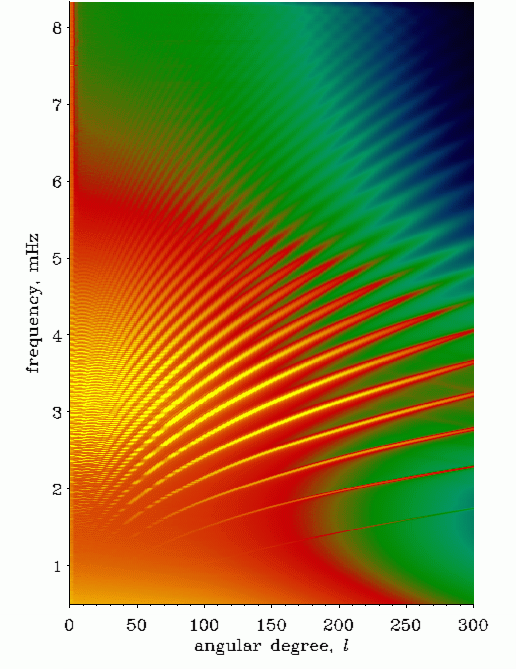
\includegraphics[width=0.8\textwidth]{pics/rhodes.png}
    \caption[Solar power spectrum from MDI]{Solar power spectrum showing helioseismic oscillation mode frequencies as a function of spherical degree as observed by MDI over a time span of $144$ days. 
    The acoustic oscillation modes of the Sun form the ridges of high power. 
        \emph{(Figure reprinted with permission from \citealt{1997SoPh..175..287R}.)}
        \label{fig:rhodes-mdi}}
\end{figure}


% Scherrer et al [134] first echelle? 
%Broomhall et al 2009, 23 years of BiSON frequencies 
%solar g-modes \citep{2010A&ARv..18..197A} 
%solar neutrino problem 
%solar internal rotation \citep{1998ApJ...505..390S, 2009LRSP....6....1H} 
%\citep{1990SoPh..128..143G} Sensitivity of solar eigenfrequencies to the age of the sun 
%\citep{1995SoPh..162..129S} SOI MDI 

\subsubsection*{Helioseismic Inversions}
Many of the confirmations of global helioseismology have come through the comparison of observations to a theoretical models constructed to match the properties of the Sun. % through e.g.~evolutionary modelling. 
Such models can be constructed for example via evolutionary modelling; I will discuss the creation of such models in more detail in Section~\ref{sec:evolution}. 
However, even to this day, no solar model matches solar oscillation data exactly \citep[e.g.,][]{1980Natur.288..544C}. 
The question thus arose as to whether these global oscillation modes could be used to make model-independent measurements of the solar interior, in terms of both its structure and its internal rotation rate \citep[e.g.,][]{1976Natur.259...89C, 1981MNRAS.196..731G}. 
%However, in part inspired by the fact that solar models did not---and still do not---fully reproduce the observed frequency spectrum, the question quickly arose whether these global oscillation modes could be used to make model-independent measurements of the solar interior, in terms of both its structure and its internal rotation rate \citep{1981MNRAS.196..731G}. 
This would need to be answered in the context of inverse theory. 
%Seeking the internal characteristics that would be most consonant with the measured oscillation frequencies. 

\epigraph{\emph{``The astrophysicists' task is not merely to produce a theoretical model of the Sun \hphantom{``}that is not obviously at variance with observation, but to learn what the internal \hphantom{``}structure actually of the Sun is, and to understand why it is so.''
}}{--- Douglas Owen Gough, FRS \\ 
\textit{Seismic observations of the solar interior} (\citeyear{1991ARA&A..29..627G})}

The forward problem of global helioseismology is to calculate the oscillation mode frequencies for a given model of solar structure (or solar rotation). 
The inverse to this problem is then to calculate the structure (or internal rotation profile) from the mode frequencies. 
The inverse problem is ill-posed because different stellar structures can support the same oscillation pattern, including ones that are clearly nonphysical. 
Furthermore, unless care is taken, small errors to the input data can lead to large errors in the inversion result. 
I will discuss ill-posed problems in more detail in Section~\ref{sec:inverse}. 
%Such frequencies can then be compared to the observed frequencies. 

In the late 1960s, geophysicists George Backus and James Gilbert developed a stable method for inferring the structure of the Earth from seismic measurements  \citep{1968GeoJ...16..169B, 1970RSPTA.266..123B}. 
This method came to be known as the Gilbert--Backus method or the method of Optimally Localized Averages (OLA) and has been adapted for use and widely applied in helioseismology. %\footnote{ There are other inversion techniques, given for example in the aforementioned review articles, but they are not relevant for the present thesis, so I omit the details here.}  
%Douglas Gough led the effort of analyzing helioseismic data using the Gilbert--Backus method (also known as the method of Optimally Localized Averages, or OLA). 

The idea of OLA is as follows. 
When comparing the model frequencies to the observed frequencies, there are differences, indicating that the structure (or rotation profile) of the model must differ from the structure of the Sun. 
%First, one compares the oscillation mode frequencies of the star to a model. 
If an oscillation mode were only sensitive to one region of the star, then a difference in frequency for that mode would indicate a difference in structure in that region. 
However, this is not the case: oscillation modes are sensitive to multiple locations in the solar interior, and so it is not possible to disentangle the cause of discrepancy based on only one mode. 

The sensitivities of mode frequencies to perturbations in the structure of the star are called kernels. 
I provide the kernels of stellar structure in Section~\ref{sec:kernels}. 
The OLA method works by combining the modes in such a way that their combination---the averaging kernel---is only sensitive to one region in the star. 
When the combination of frequencies corresponding to that combination of modes differs between the model and the star, then the structure must differ in that region. 
Thus, one can then work out the structure in the locations in the interior where it is possible to construct an averaging kernel. 
%In addition to revealing the otherwise hidden properties of the interior, inversions enable the possibility of testing the quality of theoretical models. 
%a well-localized sensitivity function, known as an averaging kernel. 
%build these sensitivity functions. 
%The OLA  star by combining the modes in such a way 
%The OLA method determines the combination of modes 


By the mid-80s, it became possible to invert frequency splittings and infer the internal rotation rate of the Sun (\citealt{1984Natur.310...22D}, see also e.g.~\citealt{1998ApJ...505..390S, 2009LRSP....6....1H}). 
The following year, the internal solar sound speed profile was deduced via inversion of an asymptotic description known as Duvall's Law, which assumes that the mode frequencies depend exclusively on the speed of sound \citep{1985Natur.315..378C}. 
%This description assumes that the mode frequencies depend exclusively on the speed of sound, which, as we will see later, is not the case. 
%In reality, the density of the stellar matter is important too. 
Soon thereafter, full inversions---which separate the influence on mode frequencies of, e.g., sound speed from density---were used to determine the acoustic structure of the majority of the solar interior (\citealt{1985SoPh..100...65G}, see also e.g.~\citealt{1990MNRAS.244..542D, GoughThompson1991, 1991ARA&A..29..627G, 1994a&as..107..421a, 2009ApJ...699.1403B}). 

Inversions for helioseismic structure have revealed many aspects of the solar interior, such as the depth of the convection zone \citep[e.g.,][]{1991ApJ...378..413C, 1997MNRAS.287..189B}, the helium abundance in the solar envelope \citep[e.g.,][]{1991LNP...388..111D, 1998MNRAS.298..719B}, the equation of state of the solar plasma \citep{1997A&A...322L...5B}, %the lack of convective undershooting \citep{1994MNRAS.267..209B}, 
and the efficiency of element diffusion \citep{1993ApJ...403L..75C}. 
Rotation inversions have shown that the Sun rotates differentially, having a latitudinally-dependent rotation rate in the convective outer envelope, and rotating as a solid body in the radiative interior \citep[e.g.,][]{2009LRSP....6....1H}. 
These zones are separated by a shear layer that is referred to as the tachocline \citep[][]{1992A&A...265..106S}. 
Finally, investigations based on helioseismic inversions have been instrumental in resolving longstanding issues such as the solar neutrino problem \citep[e.g.,][]{1998PhLB..433....1B}, for which four Nobel prizes have been awarded. 
A detailed review of results that have been obtained via helioseismic inversion has been given by \citet{2016lrsp...13....2b}. 
%The present thesis is largely a continuation of these ideas onto stars. 

%\citet{1985Natur.315..378C} inverted mode frequencies according to the asymptotic description to deduce the speed of sound throughout the solar interior. 




\subsection{Asteroseismology}
As our Sun is not thought of as being particularly exceptional, it was obviously expected that other stars similar to the Sun should also exhibit solar-like oscillations \citep[e.g.,][]{1984srps.conf...11C}. 
%Good incentives for such a discovery came from \citet{1986ApJ...306L..37U}, who argued that measured solar-like oscillations in other stars would facilitate not only the determination of their masses and radii, but also their \emph{ages}---something which so far had mainly only been possible for stellar populations. 
%This is because mode frequencies evolve with the star---not unlike rings in a tree---and so their measurement can be used to set limits on stellar ages. 
In addition to oscillations in solar-like stars, \citet{1983SoPh...82..469C} further predicted that low-mass giant stars should harbor these kinds of oscillations as well, as these stars also have convective envelopes. %meet the prerequisites for their excitation: a convective envelope. 
Moreover, these stars harbor \emph{mixed modes}: modes that behave like acoustic oscillations in the envelope and gravity mode oscillations in the core \citep[e.g.,][]{2001MNRAS.328..601D}. 
%The observation of these modes in red giants would represent a great confirmation of evolutionary theory. 
However, due to the very small amplitudes of the solar oscillations (on the order of ${10\; \text{cm/s}}$, recall Figure~\ref{fig:solar-power-spectrum}), their discovery in other stars posed a long-standing challenge. 
%\citet{1994ApJ...427.1013B} 

%$\Delta\nu$, and hence the frequencies, scales as the square root of the stellar mean density, $\Delta\nu \propto (M/R^3)^{1/2}$ (Ulrich 1986)
%$\nu_{\max} \propto \nu_{\text{ac}}$ \citep{1991ApJ...368..599B}

Already in the late 1980s detections of solar-like oscillations were being claimed \citep{1986A&A...164..383G}. 
These were not however confirmed in follow-up studies \citep[e.g.,][]{1991MNRAS.249..643I}. 
Throughout the 1990s there were more claims of detections in other stars, which mainly served to place upper limits on their amplitudes \citep[e.g.,][]{1990ApJ...350..839B, 1991ApJ...368..599B, 1992A&A...264..138P, 1995MNRAS.276.1295E}. 
%It was not until the 1990s that the first solar-like oscillations would be detected in other stars. 
%\citet{1991ApJ...368..599B} claimed indications of such oscillations in Procyon A. 
%The nature of these oscillations however remain to this day a matter of debate. 
%The first indications came, somewhat controversially, from Procyon . 
Finally, in the 2000s, firm detections of solar-like oscillations in other stars were made, such as in the nearest star, the solar-type star Alpha~Centauri \citep{2001A&A...374L...5B}; 
the subgiant star $\beta$~Hyi \citep{2001ApJ...549L.105B}; 
and the giant stars $\alpha$~Uma \citep{2000ApJ...532L.133B} and $\eta$~Hya \citep{2002A&A...394L...5F}. 
The field of solar-like asteroseismology was born, but in its infancy. 
With the coming space missions, it would soon undergo a revolution. 




%\subsubsection*{Space Asteroseismology}
The first space-based observations came from the NASA \emph{Wide-Field Infrared Explorer} (\textsc{WIRE}), which had failed in its nominal mission, but was fortunately able to be repurposed into an asteroseismology mission \citep{2000ASPC..198..557B}. 
After one month of observation, space photometry yielded solar-like oscillations in the very bright giant star Alpha~Ursae~Majoris \citep{2000ApJ...532L.133B}, and soon thereafter, in Alpha~Centauri as well \citep{2001ESASP.464..391S}. 

The first purposefully dedicated space asteroseismology mission was the Canadian \emph{Microvariability and Oscillations of STars} telescope \citep[\textsc{MOST},][duration 2003--2014]{2003PASP..115.1023W}. 
Though \textsc{MOST} was not sensitive enough to detect oscillations in solar-type stars, \citet{2006ESASP.624E..30B, 2007A&A...468.1033B} did detect radial-mode oscillations in the red giant $\epsilon$~Oph using $28$ days of MOST observations. 
Studying this same star from the ground, \citet{2006A&A...454..943H} was able to detect non-radial pulsations. 
The detection of solar-like oscillations in red giants represents a great confirmation of stellar theory. 
A detailed review on oscillations in red giants has been given by \citet{2017A&ARv..25....1H}. 
%, confirming theoretical expectations. 
%failed to detect p-modes in Procyon \citep{2004Natur.430...51M} 

\lr{Soon afterwards came the European/French space mission \emph{Convection, Rotation and planetary Transits} \citep[\textsc{CoRoT},][duration 2006--2012]{2006ESASP1306...33B}, which was able to detect solar-like oscillations in solar-type stars \citep[e.g.,][]{2010A&A...515A..87D}. 
Among other successes, CoRoT was particularly valuable for the study of solar-like oscillations in red giant stars, where oscillations in hundreds of these stars were detected (e.g., \citealt{2009Natur.459..398D, 2009A&A...506..465H}).} 


\subsubsection*{\emph{Kepler}}

By far the best asteroseismology mission to date has been the \emph{Kepler} space observatory \citep[][duration 2009--2013]{2010ApJ...713L..79K}. 
The data yield from \emph{Kepler} has been enormous; here I will largely restrict discussion to solar-type stars which are relevant for this thesis. 
For detailed reviews and textbooks on asteroseismology, see e.g.\ \citealt{2010aste.book.....a, 2012AN....333..914C, 2013adspr..52.1581h, 2013ARA&A..51..353C}, and \citealt{basuchaplin2017}. 

\emph{Kepler} targeted approximately $150,000$ main sequence stars in a fixed field of view around the constellations of Cygnus, Lyra and Draco. 
Short-cadence and long-cadence targets were observed every $58.89$ seconds and every $29.4$ minutes, respectively. 
Several pipelines were created in preparation of processing the expected asteroseismic yield. 
For example, several groups created pipelines for the automated retrieval of ${\Delta\nu}$ and $\nu_{\max}$ from \emph{Kepler} time series \citep[e.g.,][]{2009CoAst.160...74H, 2009A&A...508..877M, 2010MNRAS.402.2049H, 2010A&A...511A..46M}. 
For detailed stellar modelling, \citet{2009ApJ...699..373M} created the Asteroseismic Modelling Portal (AMP), which fits evolutionary models to the observed asteroseismic data using genetic programming. 
In a hare-and-hound exercise, \citet{2009ApJ...700.1589S} found that the radius determinations from the expected asteroseismic data from \emph{Kepler} are five to ten times better than without. 


After launch, the quality of \emph{Kepler} data for asteroseismology was immediately evident, revealing clear signatures of non-radial oscillations in several stars within one month of data collection \citep{2010PASP..122..131G, 2010ApJ...713L.169C}. 
%\citet{2010ApJ...723.1583M} used the mixed mode frequencies of a subgiant star to obtain radius and age estimates with precisions to nearly 1\%. 
For the majority of stars, only the global properties such as ${\Delta\nu}$ and $\nu_{\max}$ are able to be resolved. 
Even with just these quantities, however, it is possible to infer information about the stars. 
For example, by assumption of homology with the Sun, one can scale oscillation data from solar values to estimate the properties of stars, such as their masses and radii \citep[e.g.,][]{1995A&A...293...87K}. %can use ``solar scaling relations'' to estimate the mass and radius of a star. 
This presents the opportunity for ``ensemble asteroseismology.''
%Even with just these quantities, such stars present the opportunity for ``ensemble'' asteroseismology. 
\citet{2011Sci...332..213C, 2014ApJS..210....1C} and \citet{2017ApJS..233...23S} used these and other approaches to find the masses, ages, radii, and other fundamental parameters for hundreds of main sequence and subgiant stars observed by \emph{Kepler}. 
In addition, several groups have also worked on improvements to the solar scaling relations \citep[e.g.,][]{2013A&A...550A.126M,2016ApJ...822...15S,2016MNRAS.460.4277G,2017MNRAS.470.2069G,2017ApJ...843...11V}. 

For the best targets, interferometric and spectroscopic measurements have been obtained to complement the asteroseismic data \citep[e.g.,][]{2010MNRAS.405.1907B, 2012MNRAS.423..122B, 2012ApJ...749..152M, 2013MNRAS.433.1262W}. 
%These targets have masses and radii claimed to better than $1\%$ precision and ages to better than $3\%$ precision. 
These measurements provide the tightest determinations of stellar parameters and the best tests to stellar theory. 
Comparing these data, \citet{2012ApJ...760...32H} found good agreement between radii determined via interferometry and asteroseismology. 
\begin{figure}
    \centering
    \includegraphics[width=\linewidth]{figs/pgrams/cygb_lc.pdf}\\
    \includegraphics[width=\linewidth]{figs/pgrams/cygb_pgram.pdf}
    %\includegraphics[width=0.5\textwidth]{ch1_introduction/%pics/cygb_lc.pdf}%
    %\includegraphics[width=0.5\textwidth]{ch1_introduction/%pics/cygb_pgram.pdf}
    \caption[Power spectrum of 16~Cyg~B]{
        Light curve (top) and power spectrum of 16~Cyg~B (bottom) as obtained from the \emph{Kepler} spacecraft. 
        %Each of the 56 peaks in the power spectrum correspond to an individual mode of oscillation. 
        The power spectrum shows $56$ detected oscillation modes, each labelled by their spherical degree (\emph{cf.}~Figure~\ref{fig:sph}). 
        The power excess is roughly Gaussian in shape and centered around a value of ${\nu_{\max}\simeq 2550 \;\mu\text{Hz}}$. 
        The inset figure shows a zoom into the power spectrum with example large (${\Delta\nu \simeq 117\;\mu\text{Hz}}$) and small (${\delta\nu \simeq 6\;\mu\text{Hz}}$) frequency separations. 
        \emph{Data from the Kepler Asteroseismic Science Operations Center \citep{KASOC}.}
    \label{fig:16cygb}}
\end{figure}


The perhaps best solar-like stars observed by \emph{Kepler} are the solar analogs 16~Cygni~A and B. 
These stars form a hierarchical triple system, with 16~Cyg~A being orbited by a red dwarf, and 16~Cyg~B being orbited by a Jovian planet.  %which reside in a triple system along with a red dwarf 16~Cygni~C. 
\citet{2012ApJ...748L..10M} ``peak bagged'' these stars (i.e., resolved their frequencies) and found clear detections of ${\ell\leq 3}$ modes (see Figure~\ref{fig:16cygb}). 
%, and then used AMP to determine their fundamental parameters. 
They used AMP to determine the evolutionary parameters of these stars, finding a common age of $6.8$~Gyr and common initial chemical compositions, which supports the conatality hypothesis of binary star formation. 
%Follow-up studies have found similar ages \citep[e.g.,][]{2013MNRAS.435..242G, }
\citet{2015MNRAS.446.2959D} used rotational splittings of the non-radial modes to infer the inclination angles and rotation rates of these stars, in both cases finding a rotation rate of approximately $23$~days. 


For approximately $100$ solar-like stars observed by \emph{Kepler}, the data have been good enough for dozens of individual mode frequencies to be resolved. 
These stars form the \emph{Kepler} Ages \citep{2016MNRAS.456.2183D} and \emph{Kepler} LEGACY projects \citep{2017ApJ...835..172L}, the former of which comprises $35$ planet-host candidates. 
\citet{2015MNRAS.452.2127S, 2017ApJ...835..173S} determined the fundamental parameters of these stars using pipelines created by different groups, finding roughly broad agreement. 
%The former consists of 35 planet-host candidates.
%\citet{2017A&A...608A.112N} followed up these observations with high-resolution spectroscopy and confirmed that 
\citet{2014ApJ...790..138V, 2017ApJ...837...47V} used seismic glitch analysis to determine the base of the convection zone and helium abundances for the LEGACY sample.
These are the stars analyzed in the coming Sections and Chapters.  





A discussion of the \emph{Kepler} mission would be incomplete without a mention of exoplanets. 
\emph{Kepler} was primarily a plunt-hunting mission, and a very successful one. 
Within \emph{Kepler} data researchers found a plethora of rocky planets, super Earths, and gas giants \citep[e.g.,][]{2008ApJ...680.1450P, 2011ApJ...729...27B, 2012ApJ...745..120B, 2014ApJS..210...20M}. 
Additionally, \emph{Kepler} data were used to find that hot Jupiters are common \citep{2008ApJ...680.1450P}, and that many stellar-planetary systems are misaligned \citep{2013Sci...342..331H}, bringing into question theories of planet formation. 
Of course, asteroseismology is of great aid to the characterization of exoplanets, since the determination of exoplanetary parameters usually depends strongly on the ability to determine the parameters of the host star (see Figure~\ref{fig:exoplanets}). 

\begin{figure}
    \centering
    \begin{minipage}[c]{0.5\textwidth}%
        %\frame{%
        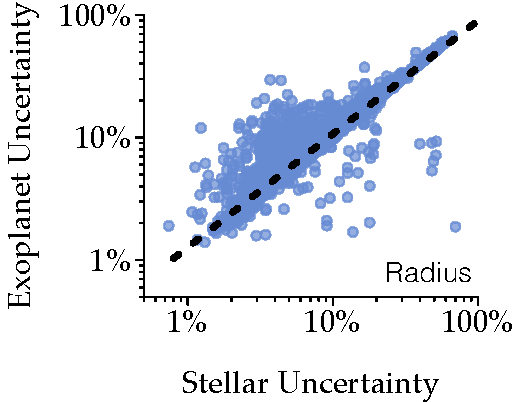
\includegraphics[width=\textwidth]{figs/exo-radius.pdf}%
        %}
    \end{minipage}%
    %\hspace*{0.05\textwidth}%
    \hfill
    \begin{minipage}[c]{0.45\textwidth}
        \caption[Exoplanetary uncertainty vs.~host star uncertainty]{Uncertainty in the determination of exoplanetary radii as a function of the uncertainty in the determination of the radius of their host star for nearly $2,400$ exoplanets detected using the transit method, which will also be the method of choice for finding exoplanets in the forthcoming TESS mission. 
        %Stellar uncertainty is the principal source of exoplanetary uncertainty. 
        %\newline\newline
        \emph{Data acquired from \href{http://exoplanets.org}{exoplanets.org} \citep{2014PASP..126..827H}.}
        \label{fig:exoplanets}}
    \end{minipage}
    %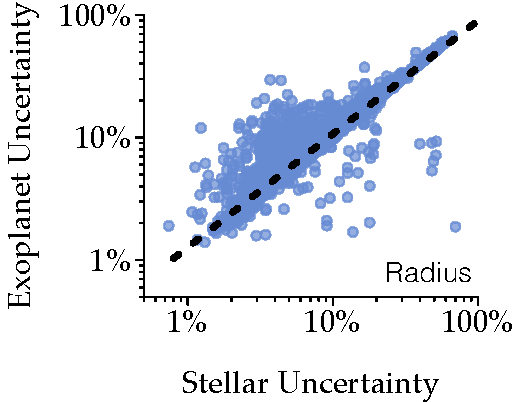
\includegraphics[width=.5\textwidth]{figs/exo-radius.pdf}
    %\caption{Uncertainty in the determination of exoplanetary radii as a function of the uncertainty in the determination of the radius for their host star for nearly $2,400$ exoplanets detected using the transit method. 
    %\emph{Data acquired from \href{http://exoplanets.org}{exoplanets.org} \citep{2014PASP..126..827H}.}
    %\label{fig:exoplanets}}
\end{figure}

Following the failure of its reaction wheels, \emph{Kepler} was repurposed into the wandering K2 mission, which is now in its final stages \citep[][duration 2013--2018]{2014PASP..126..398H}. 
This year, NASA's \emph{Transiting Exoplanet Survey Satellite} mission will launch \citep[TESS,][expected 2018--2020]{2010AAS...21545006R}. 
ESA's \emph{Planetary Transits and Oscillations of stars} mission \citep[PLATO,][expected 2026--2030]{2014ExA....38..249R} is planned for launch in eight years. 
We analyze the anticipated yields of these missions for Sun-like stars in Chapter~\ref{chap:statistical} \citep{2017apj...839..116a}. 



\subsubsection*{Asteroseismic Inversions}

Asteroseismic structure inversions are more difficult to perform than in helioseismology for two main reasons. 
\begin{description}
    \setlength{\itemindent}{0pt}
    \item[Mode set.]
    The mode sets available in asteroseismology are much more limited. 
    Due to cancellation effects, only low-degree modes have been observed so far in stars other than the Sun, and so only dozens rather than thousands of mode frequencies are available. 
    \lr{It is only possible to build well-localized averaging kernels in locations where there is a sufficient number of mode lower turning points, as these are the regions where the modes spend most of their time (recall Figure~\ref{fig:rays}). 
    Consequently, asteroseismic inversions using only low-degree modes are generally only capable of making localized probes of the stellar core.} 
    This limitation also rules out the possibility of using techniques such as Regularized Least Squares, which fit the entire internal profile simultaneously \citep[see, e.g.,][]{basuchaplin2017}. 
    
    Furthermore, mode frequencies depend on multiple variables of stellar structure.
    When trying to determine one from asteroseismic information, one must therefore control for other influences. 
    With limited information, this becomes more difficult. 
    In helioseismology, the most common pair of variables is the speed of sound $c$ and the stellar density $\rho$, denoted the ${(c,\rho)}$ kernel pair. 
    
    \item[Mass and radius.]
    The masses and radii of stars are not known to anywhere near the precision for the Sun. 
    This creates difficulties because the kernel functions are derived with respect to a reference model, which is assumed to have the correct mass and radius. 
    Without accounting for this effect, the results of the inversion results will be offset by the differences in mass and volume \citep[][]{2003Ap&SS.284..153B}. 
    Furthermore, the mode frequencies themselves scale with the mass and volume of the star. 
    %These effects need to be accounted for when performing asteroseismic inversions. 
\end{description}

Already in the early 1990s, before the first confirmed asteroseismic detections, \citet{1993ASPC...40..541G} considered the prospect of performing asteroseismic inversions to determine stellar structure. 
In this work, Gough and Kosovichev simulated data sets for a $1.1$ solar mass model that they thought might be likely to be obtained from a future mission. %the PRISMA mission. 
They used a solar model as reference. 
%, and simultaneously estimated the difference in the ratio of mass per volume. 
%They inverted for the structure of the proxy star using a solar model as reference. 
Their work was on the one hand pessimistic---assuming only ${\ell\leq 2}$ modes would be available, having mode uncertainties of ${0.1\;\mu\text{Hz}}$---and on the other optimistic, assuming that more than $60$ modes would be observed. 
In comparison, the perhaps best \emph{Kepler} solar-type target, 16~Cyg~B, has approximately $56$ detected modes (though the exact amounts are disputed), $11$ of which being ${\ell=3}$ modes, with uncertainties ranging from ${0.04\;\mu\text{Hz}}$ up to ${5\;\mu\text{Hz}}$. 

Gough and Kosovichev were able to form four well-localized averaging kernels at target radii $0.05$, $0.15$, $0.25$, and $0.35$. 
They simultaneously estimated the difference in mass per volume between the two models while performing the inversion. 
Surface effects were not considered. 
%Unfortunately, the PRISMA mission was not funded. 

In this work it was already realized that inversions with helium as the second variable could be the most promising route. 
The helium kernels only have amplitude in ionization zones, which are located near to the stellar surface and would require higher-degree modes to resolve anyway. 
\citet{2001ESASP.464..407B} showed that when using the ${(c,\rho)}$ kernel pair with expected asteroseismic data, only one averaging kernel can be formed. 

Some other early attempts with similar setups and results have been reviewed by \citet{2003Ap&SS.284..153B}. 
These works all used mode sets that they thought would be available from future missions: PRISMA, MOST, MONS, and \emph{Eddington}. %, and CoRoT. 
\lr{Unfortunately, PRISMA, MONS, and \emph{Eddington} were not funded, and MOST did not detect any oscillations in solar-like stars. %; and save for perhaps a couple of stars, the observing strategy of CoRoT was not conducive to producing the quality of data that is required for asteroseismic structure inversions.} 
It is only now with the CoRoT and \emph{Kepler} missions that the data are good enough to measure internal stellar structure.} 
We invert \emph{Kepler} data to infer the internal structure of 16~Cyg~A and B in Chapter~\ref{chap:inversion} \citep{2017ApJ...851...80B}. 

%inversion differential response 
%\citep{2002ESASP.485..341R} 
%inversion for internal rotation rates of 6 stars \citep{2014A&A...564A..27D} 

Several other kinds of inverse problems have been worked on using asteroseismic data. 
Instead of inverting for the full density profile, \citet{2012A&A...539A..63R} introduced an OLA-based technique for estimating stellar mean density. 
They applied the technique to the Sun, $\alpha$~Cen~B, and two stars observed by CoRoT. 
They found that they could estimate mean densities this way to an accuracy of $0.5\%$. 
However, it performed no better than estimating mean densities using the \citet{2008ApJ...683L.175K} surface term corrected solar scaling relation. 
%Though this technique is more accurate than the ordinary $\Delta\nu$ scaling relation, it performed no better at estimating mean densities after correcting for the surface term using the relation of \citet{2008ApJ...683L.175K}. 

\citet{2015A&A...583A..62B, 2015A&A...574A..42B} extended this work by creating kernels for the acoustic radius and two age indicators: the integral of the sound speed derivative, and a weighted square of the isothermal sound speed derivative. 
%\citet{2015A&A...583A..62B} created an additional age indicator based off a weighted square of the isothermal sound speed derivative. 
They applied these techniques to 16~Cyg~A and B, and, when combining them with interferometric radii, found masses and ages for these stars that were inconsistent with evolutionary modelling \citep{2016A&A...585A.109B, 2016A&A...596A..73B}. 

In addition to the global properties of stars, inversions for stellar rotation rates have also had success. 
\citet{2012ApJ...756...19D, 2014A&A...564A..27D}, \citet{2016ApJ...817...65D}, and \citet{2017A&A...602A..62T} inverted frequency splittings to obtain the core and envelope rotation rates of several sub- and red-giant stars. 
They found, in agreement with theoretical expectations, that the cores of these stars rotate more rapidly than their outer layers. 

\newpage
\subsubsection*{Layout of Thesis}
In this section, we saw that the study of pulsating stars has been a primary driver in the development of the theory of stellar evolution. 
Helioseismic inversions have revealed the structure of the Sun and shown that it is very close (though not identical to) the structure predicted by theoretical models. 
Asteroseismology has confirmed many details predicted by stellar evolution, and asteroseismic inversions show promise for leading to future improvements to evolutionary theory. 

For the interested reader, the following texts contain more details: 
\citet{1958HDP....51..353L} give a thorough overview of variable stars up until the 1950s; 
\citet{ARNY1990211} gives the history of stellar evolution, including later phases of evolution which are not covered here; 
\citet{2016lrsp...13....2b} gives the history of solar oscillations;
\citet{bolt2007biographical} contains an encyclopedia of biographies for astronomers;
and \citet{2015pust.book.....C} give a general overview and history of variable stars.

The remainder of the thesis is organized as follows. 
The following two sections (\ref{sec:evolution}, \ref{sec:pulsation}) give the theoretical background on stellar structure, evolution, and pulsation. 
These enable us to pose and solve the forward problems of simulating the evolution of a star and calculating its frequencies of oscillation. 
In Section~\ref{sec:pulsation}, I furthermore state the kernel functions of stellar structure, which allow us to calculate the differences in mode frequencies between a pair of stellar models of differing structure. 
In the final section of the introduction (Section~\ref{sec:inverse}), I state more formally the inverse problems of asteroseismology that are considered in this thesis, and give some indication of their difficulty. 

In Chapter~\ref{chap:ML}, we perform evolution inversions to determine stellar ages and other fundamental parameters using machine learning \citep{2016apj...830...31b}. 
In Chapter~\ref{chap:statistical}, we use unsupervised machine learning to determine which observations are useful for constraining which properties of stellar models \citep{2017apj...839..116a}. 
In Chapter~\ref{chap:inversion}, we determine the asteroseismic structure of two stars, in one case finding agreement with evolutionary modelling, but in another not \citep{2017ApJ...851...80B}. 
Finally, at the end I give what I assess to be the future prospects for this line of research. 





%The data were good enough to resolve exoplanet atmospheres, and even to find tracers of water therein \citep{2017AJ....153..138B}. 
%\subsubsection*{Exoplanets}
%Kepler's first rocky planet \citep{2011ApJ...729...27B}
%Masses, Radii, and Orbits of Small Kepler Planets: The Transition from Gaseous to Rocky Planets \citep{2014ApJS..210...20M}
%Kepler-22b: A 2.4 Earth-radius Planet in the Habitable Zone of a Sun-like Star \citep{2012ApJ...745..120B}
%discovery of hot jupiters (51 Peg b) \citep{1995Natur.378..355M} and they're common \citep{2008ApJ...680.1450P} and it has water in its atmosphere \citep{2017AJ....153..138B}
%stellar spin-orbit misalignment in a multiplanetary system \citep{2013Sci...342..331H} 
%One person's trash is another's treasure: reduction in stellar oscillation and granulation for planetary studies \citep{2011A&A...525A.140D}

%The first asteroseismology results from CoRoT came in 2008 for an F-type star \citep{2008A&A...488..705A}. 
%By 2010, CoRoT had detected solar-like oscillations in a solar-type star \citep{2010A&A...515A..87D}. 
%It was not until 2010 that CoRoT detected solar-like oscillations in a solar-type star 

%Finally came \emph{Kepler} \citep[][2009--2013]{2010ApJ...713L..79K}. 
    %150,000 targets
    %correcting light curves for instrumental effects \citep{2011MNRAS.414L...6G}
    %Kepler asteroseismology program \citep{2010PASP..122..131G}
    %Kepler input catalog \citep{2011AJ....142..112B}
    %10x better stellar radii \citep{2009ApJ...700.1589S}

%K2 mission \citep[][2013--2018]{2014PASP..126..398H}
%textbooks on asteroseismology: \cite{2010aste.book.....a} and \cite{basuchaplin2017}. 
%interferometry of $\alpha$ Cen \citep{2003A&A...404.1087K}
%Detection of Solar-like oscillations in the G7 giant star 
%Houdek and Gough 2006 asteroseismic signature of helium ionization 
%inclination angles from asteroseismology \citep{2003ApJ...589.1009G} 

%\subsubsection*{Asteroseismic Inversions}

%\citet{2014A&A...564A..27D} and  found similar results when subsequently applying this method to $7$ more subgiants and red giants. 

%Using seismic inversions to obtain an indicator of internal mixing processes in main-sequence solar-like stars \citep{2015A&A...583A..62B}
%Constraints on the structure of 16 Cygni A and 16 Cygni B using inversion techniques \citep{2016A&A...585A.109B}
%Stellar acoustic radii, mean densities, and ages from seismic inversion techniques \citep{2015A&A...574A..42B}
%Constraining convective regions with asteroseismic linear structural inversions \citep{2015A&A...574A..42B}
%In-depth study of 16CygB using inversion techniques \citep{2016A&A...596A..73B}
%Estimating stellar mean density through seismic inversions 




%The remainder of the targets generally 


%\citet{2015MNRAS.446.2959D} and \citet{2017ApJ...835..172L} ``peak bagged'' these stars; i.e., determined their mode frequencies. 
%and that the masses of 16~Cyg~A and B are 8\%
%Kjeldsen et al 2008 surface effect corrections
%Stello et al 2009 relation between Dnu and numax 
%Revised Stellar Properties of Kepler Targets for the Quarter 1-16 Transit Detection Run \citep{2014ApJS..211....2H}
%good agreement with interferometry \citep{2012ApJ...760...32H}
%gyrechronology \citep{2014A&A...572A..34G}
%\subsubsection*{Solar-like Stars}
%Asteroseismic Diagrams from a Survey of Solar-like Oscillations with Kepler \citep{2011ApJ...742L...3W}
%first kepler results: 20 modes in 3 solar-like stars \citep{2010ApJ...713L.169C}
%Ensemble Asteroseismology of 500 Solar-Type Stars with the NASA Kepler Mission \citep{2011Sci...332..213C}
%Silva Aguirre et al 2011 constraining mixing in stellar cores 
%Silva Aguirre et al 2011 one-solar mass evolutionary sequence from Kepler 
%accurate parameters for 23 stars interferometry+spectroscopy+asteroseismology \citep{2010MNRAS.405.1907B} and then 93 stars \citep{2012MNRAS.423..122B}
%magnetic activity cycle in a sun-like star \citep{2010Sci...329.1032G}
%masses and radii to 1\%, ages to 2.5\% \citep{2012ApJ...749..152M}
%AMP applied to 16 Cygni \citep{2012ApJ...748L..10M}
%\subsubsection*{Sub-giant Stars}
%Deheuvels et al 2011 subgiants mixed modes 
%\subsubsection*{Red-giant Stars}
%review on red giants \citep{2017A&ARv..25....1H}. 
%CoRoT increase the number of G-K giant stars for which solar-like oscillations are observed by a factor of 100 \citep{2009A&A...506..465H}
%non-radial oscillation modes with long lifetimes in giant stars \citep{2009Natur.459..398D}. 
%universal red giant oscillation pattern \citep{2011A&A...525L...9M} 
%Mixed modes in red-giant stars observed with CoRoT \citep{2011A&A...532A..86M}
%Solar-like Oscillations in Low-luminosity Red Giants: First Results from Kepler \citep{2010ApJ...713L.176B}
%Period-luminosity relations in evolved red giants explained by solar-like oscillations \citep{2013A&A...559A.137M}
%Gravity modes as a way to distinguish between hydrogen- and helium-burning red giant stars \citep{2011Natur.471..608B}
%Spin down of the core rotation in red giants \citep{2012A&A...548A..10M}
%red giant in a binary \citep{2010ApJ...713L.187H}
%70\% of red giants show solar-like oscillations \citep{2011MNRAS.414.2594H}
%period spacings \citep{2012A&A...540A.143M}
%spectroscopy and asteroseismology for 1916 stars APOKASC \citep{2014ApJS..215...19P}
%\subsubsection*{Stellar Populations}
%red giants in open clusters \citep{2011A&A...530A.100H, 2012ApJ...757..190C, 2012A&A...543A.106B, 2011ApJ...729L..10B}
%mass loss old open cluster \citep{2012MNRAS.419.2077M}
%\subsubsection*{Galactic Archeology}
%mapping and dating stellar populations with asteroseismology of red-giant stars \citep{2013MNRAS.429..423M}
%separation of red giant branch, red clump, and secondary clump for 13,000 giants \citep{2013ApJ...765L..41S}